% !TeX root = ../main.tex
\chapter{DEVELOPMENT AND IMPLEMENTATION PLAN}

\section{Chapter Objectives}
This chapter presents the development and implementation plan of the Web-Based Cyber Range platform. The objective is to translate the architectural decisions and system requirements into an executable implementation path that is technically coherent, operationally feasible, and aligned with the capstone project context. Rather than presenting isolated technical components, this chapter explains how the platform was constructed as an integrated system centered on dashboard-driven orchestration.

The implementation narrative focuses on how infrastructure providers, reusable templates, scenario definitions, deployment workflows, asynchronous task processing, and monitoring views were progressively integrated into a unified control environment. The chapter also clarifies implementation sequencing, milestone logic, quality control practices, and operational risk management used to deliver a stable academic prototype.

\section{Implementation Strategy}
\subsection{Development Approach}
The system was developed using an incremental and workflow-oriented approach. This approach was selected because the platform includes tightly connected subsystems: provider configuration, resource templating, scenario lifecycle management, asynchronous execution, and dashboard interaction. Implementing all modules simultaneously would have introduced high integration risk and low observability during debugging. Therefore, the team implemented and validated each functional layer in sequence, while preserving compatibility with subsequent phases.

A key design decision was the separation between the control layer and the execution layer. The control layer manages configuration, orchestration, authorization, and user interaction through the dashboard and backend services. The execution layer performs environment provisioning and scenario runtime operations through asynchronous jobs and resource actions. This separation reduces coupling, improves fault isolation, and allows operational events to be traced more clearly in task and log views.

Within this architecture, the dashboard serves as the central coordination interface. It is not merely a visualization surface; it is the operational entry point through which users configure providers, manage templates, define scenarios, trigger deployments, and monitor execution outcomes. This dashboard-centric workflow ensures consistency between user intent, backend orchestration, and runtime system state.

\subsection{Work Breakdown Structure}
The implementation was organized into seven functional work streams: infrastructure provider setup, template and resource preparation, scenario definition and management, scenario deployment and execution, monitoring and task management, dashboard interaction and visualization, and AI-assisted analysis integration. This structure was chosen to reflect real operational dependencies instead of abstract technical categories.

The first three work streams establish controllable inputs: verified provider access, reusable environment artifacts, and scenario definitions. The next two work streams execute and supervise runtime behavior: deployment orchestration, task-state tracking, and log interpretation. The final work streams deliver usability and analytical value through dashboard interaction and AI-assisted interpretation where available. This decomposition provided clear ownership boundaries while preserving end-to-end system continuity.

\subsection{Technology Stack Alignment}
Technology selection was guided by operational requirements rather than by framework preference. The backend stack supports persistent configuration management, scenario lifecycle control, and asynchronous task execution for long-running deployment actions. The data layer supports both structured state management and job-status tracking. The frontend dashboard provides user-facing orchestration and monitoring views that align with backend workflows.

At the security and monitoring level, the platform integrates telemetry-oriented components so that deployment and scenario activity can be observed, diagnosed, and validated. Where AI-assisted analysis is enabled, it is positioned as a supporting interpretation layer over system outputs, not as a replacement for deterministic system control. This alignment ensures that each technology contributes directly to controllability, traceability, and educational usefulness in the Cyber Range environment.

\section{System Development Phases}
\subsection{Phase 1: Infrastructure Provider Setup}
The objective of this phase was to establish a trusted connection between the control platform and infrastructure providers. Core functions included provider profile creation, credential handling, connection validation, and persistence of provider configuration for reuse in later lifecycle operations.

This phase plays a foundational role because all downstream provisioning and scenario operations depend on reliable provider connectivity. Without validated provider integration, template operations and deployment workflows cannot be executed predictably.

The practical onboarding workflow used in this project is documented in the screenshot sequence under \texttt{images/infra}. The implementation procedure is as follows:

\begin{enumerate}
    \item Navigate to \texttt{Infrastructure $\rightarrow$ Providers}, then select \texttt{Add Provider}.
    \item Select \texttt{Proxmox VE} as provider type.
    \item Fill provider metadata and connection fields, including display name, host, API port, SSL policy, and API token.
    \item Continue setup wizard to bind runtime infrastructure options: Proxmox node, Internet bridge, ISO storage, and VM storage.
    \item Confirm setup and validate provider status until it appears as \texttt{Configured} and \texttt{Active}.
\end{enumerate}

\begin{figure}[H]
    \centering
    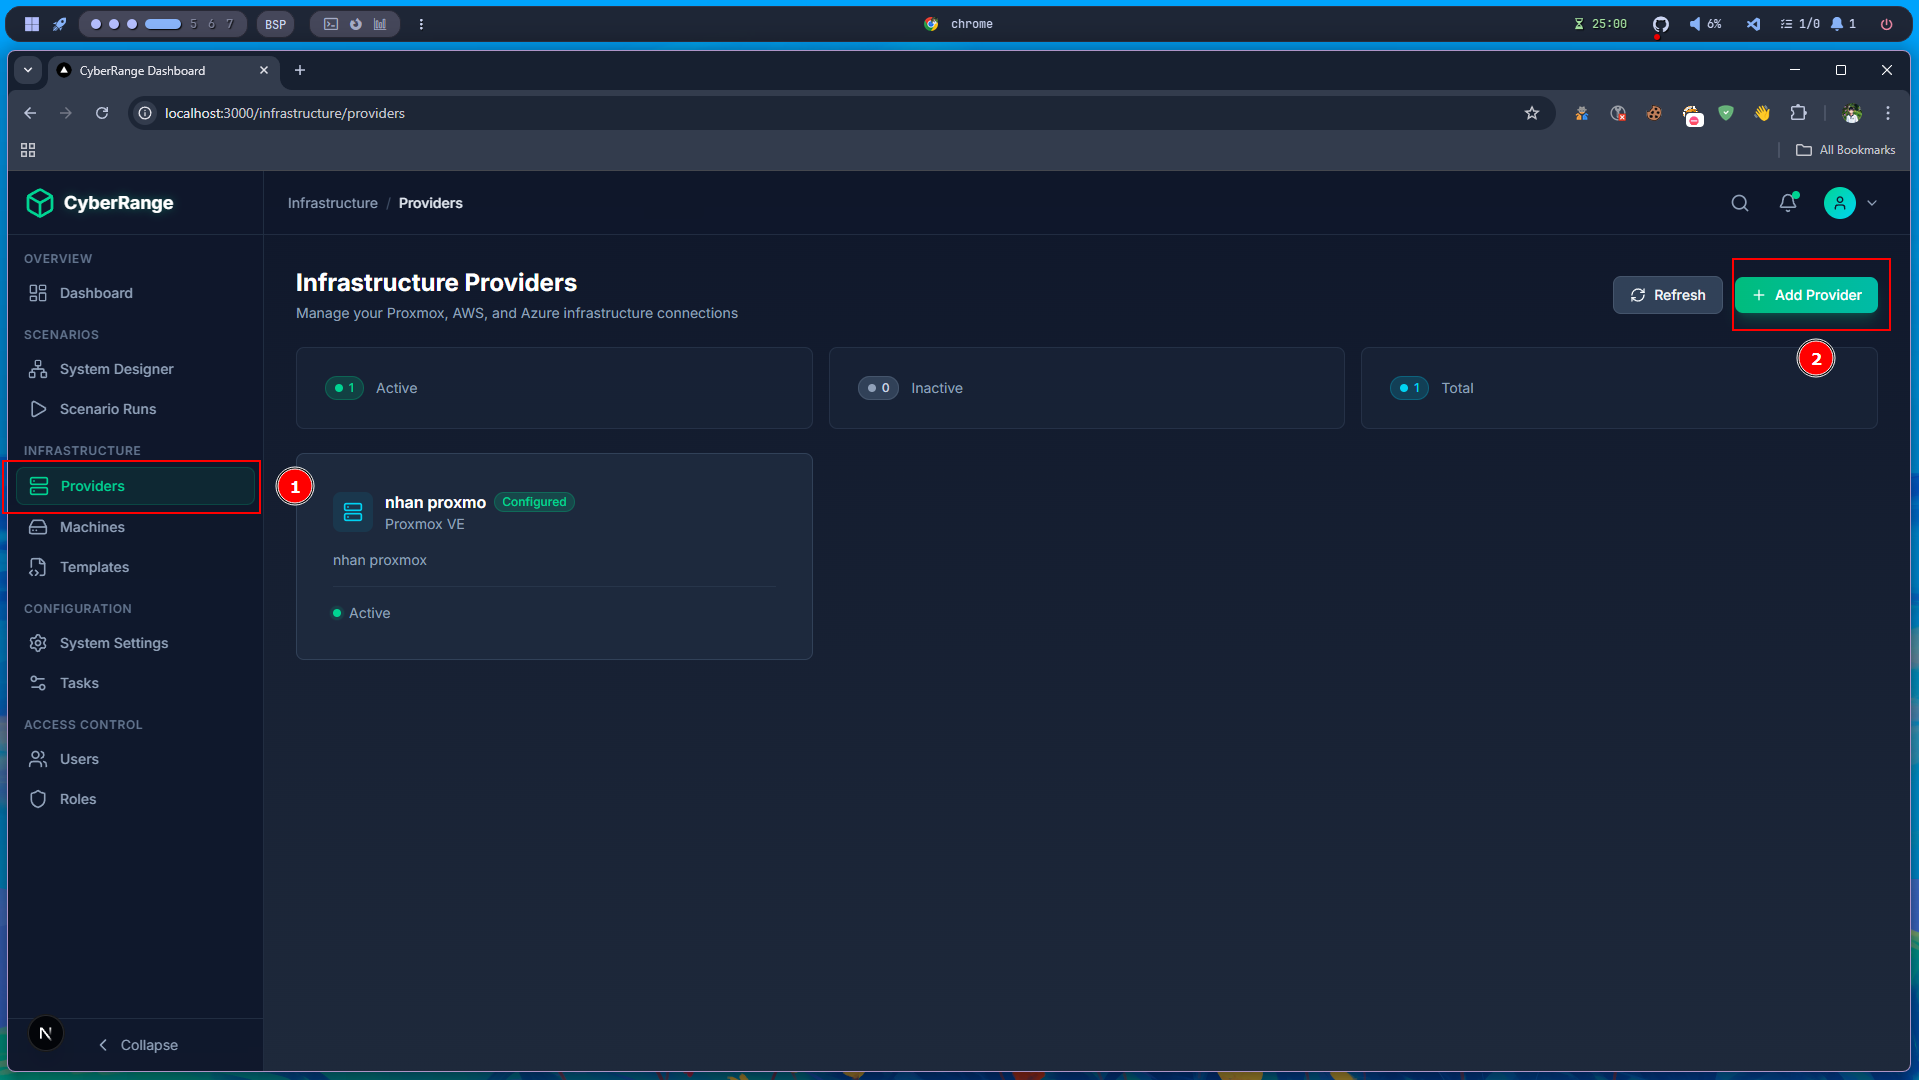
\includegraphics[width=0.95\textwidth]{images/infra/1.png}
    \caption{Provider list view.}
    \label{fig:infra-provider-list}
\end{figure}

\begin{figure}[H]
    \centering
    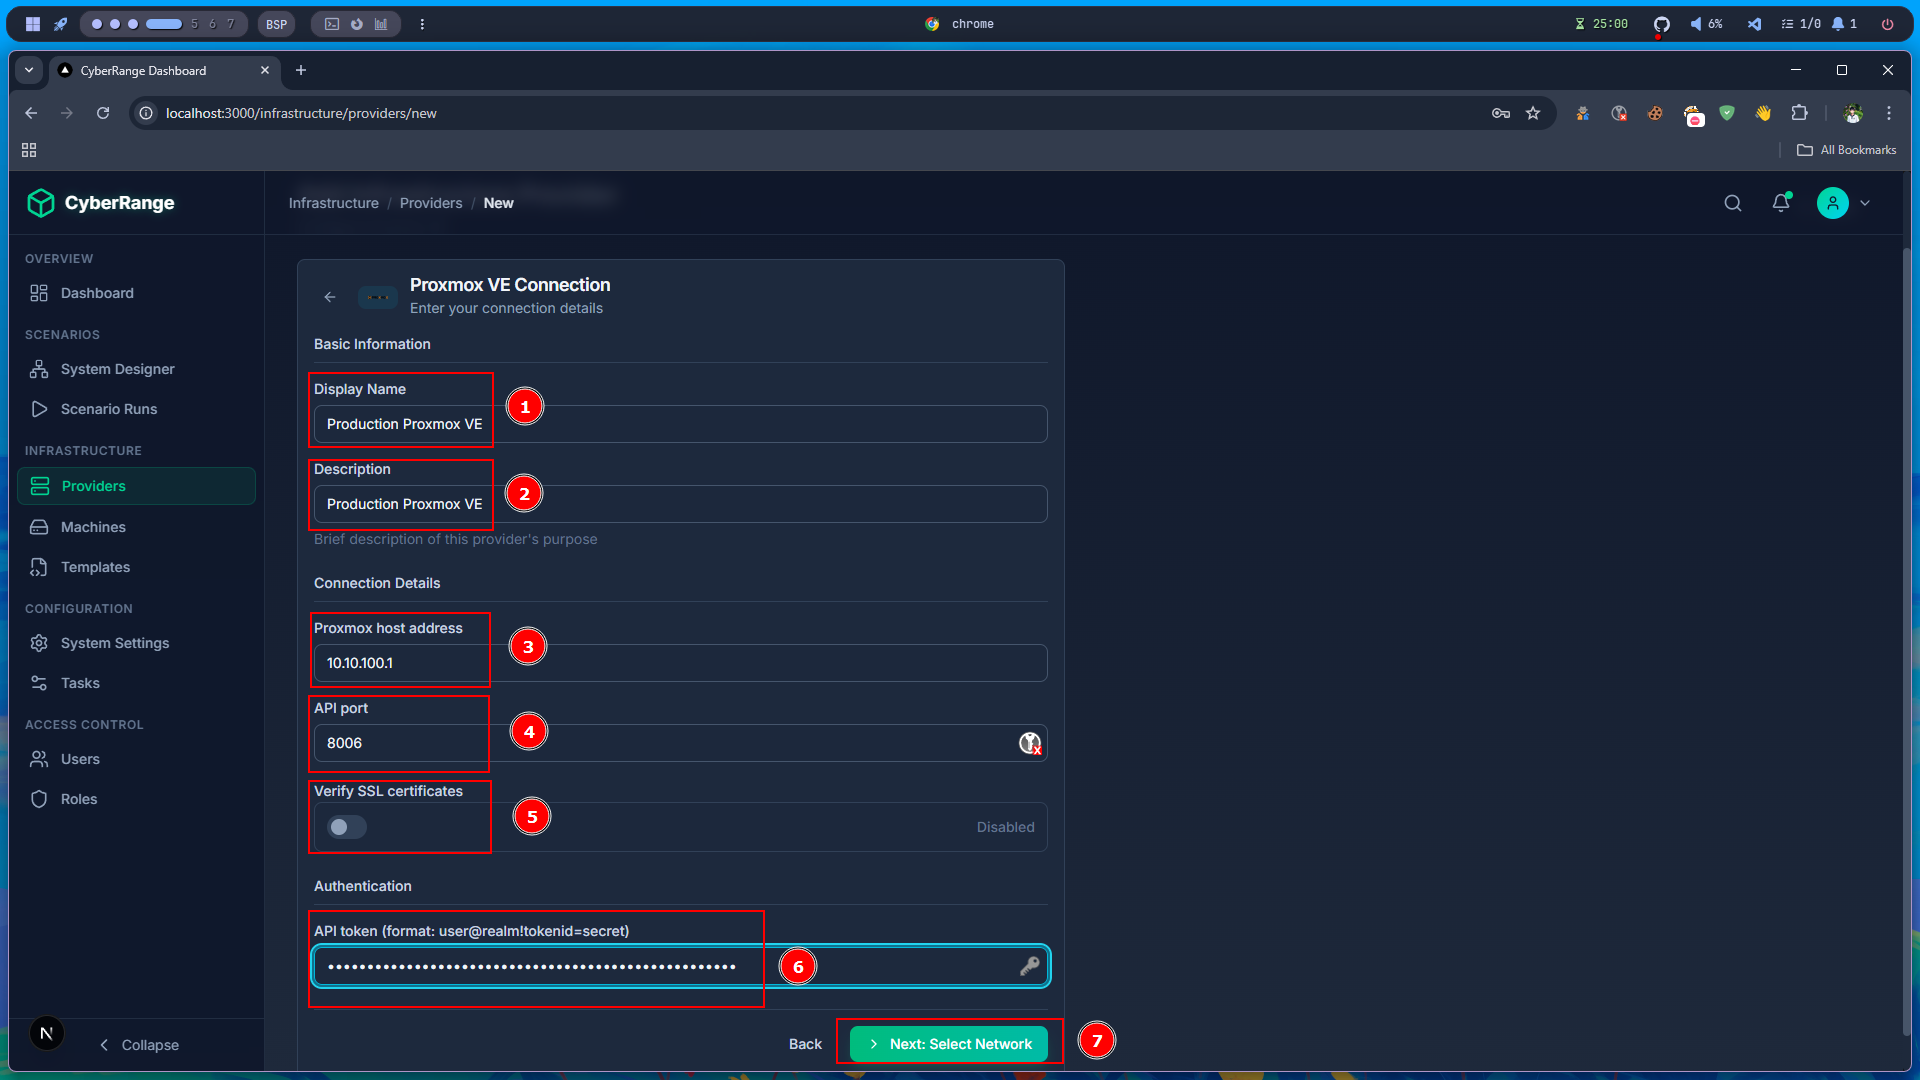
\includegraphics[width=0.95\textwidth]{images/infra/3.png}
    \caption{Proxmox connection form.}
    \label{fig:infra-provider-connection-form}
\end{figure}

\begin{figure}[H]
    \centering
    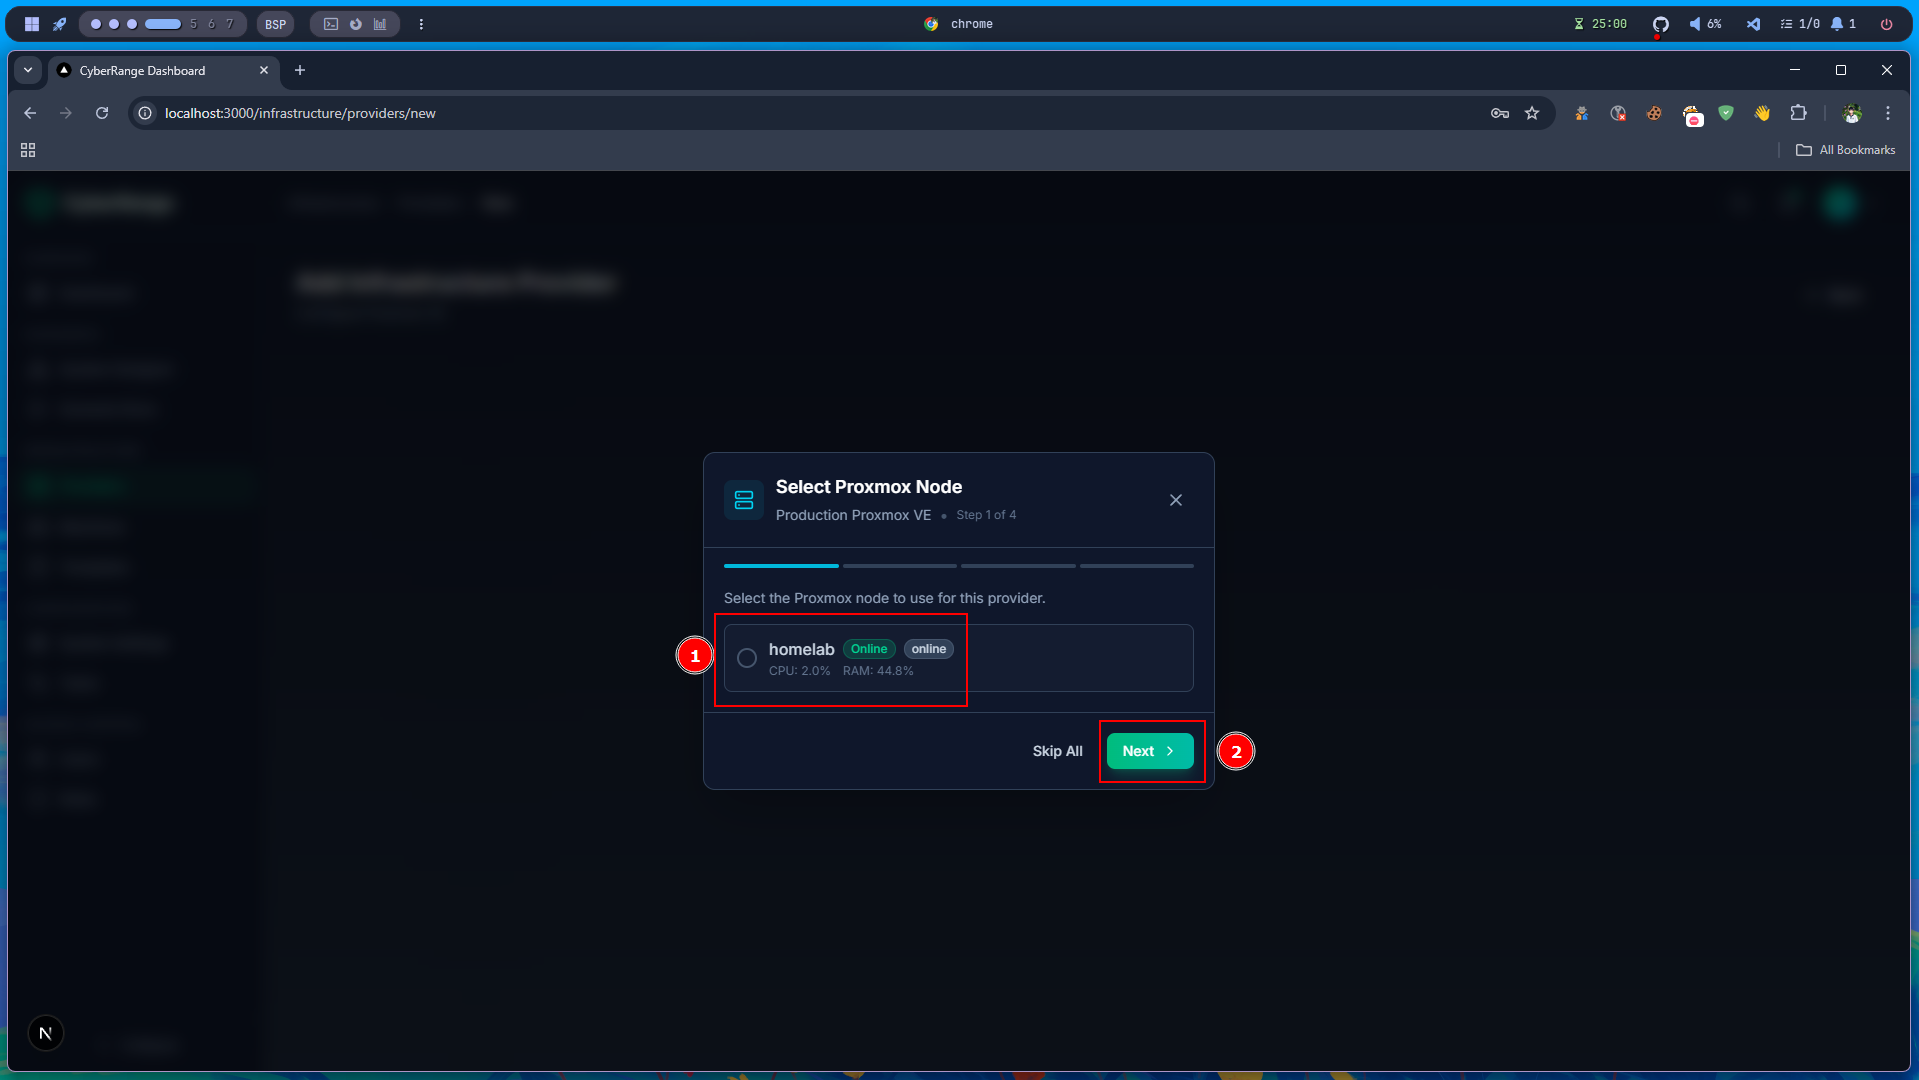
\includegraphics[width=0.95\textwidth]{images/infra/4.png}
    \caption{Proxmox node selection.}
    \label{fig:infra-provider-node-step}
\end{figure}

\begin{figure}[H]
    \centering
    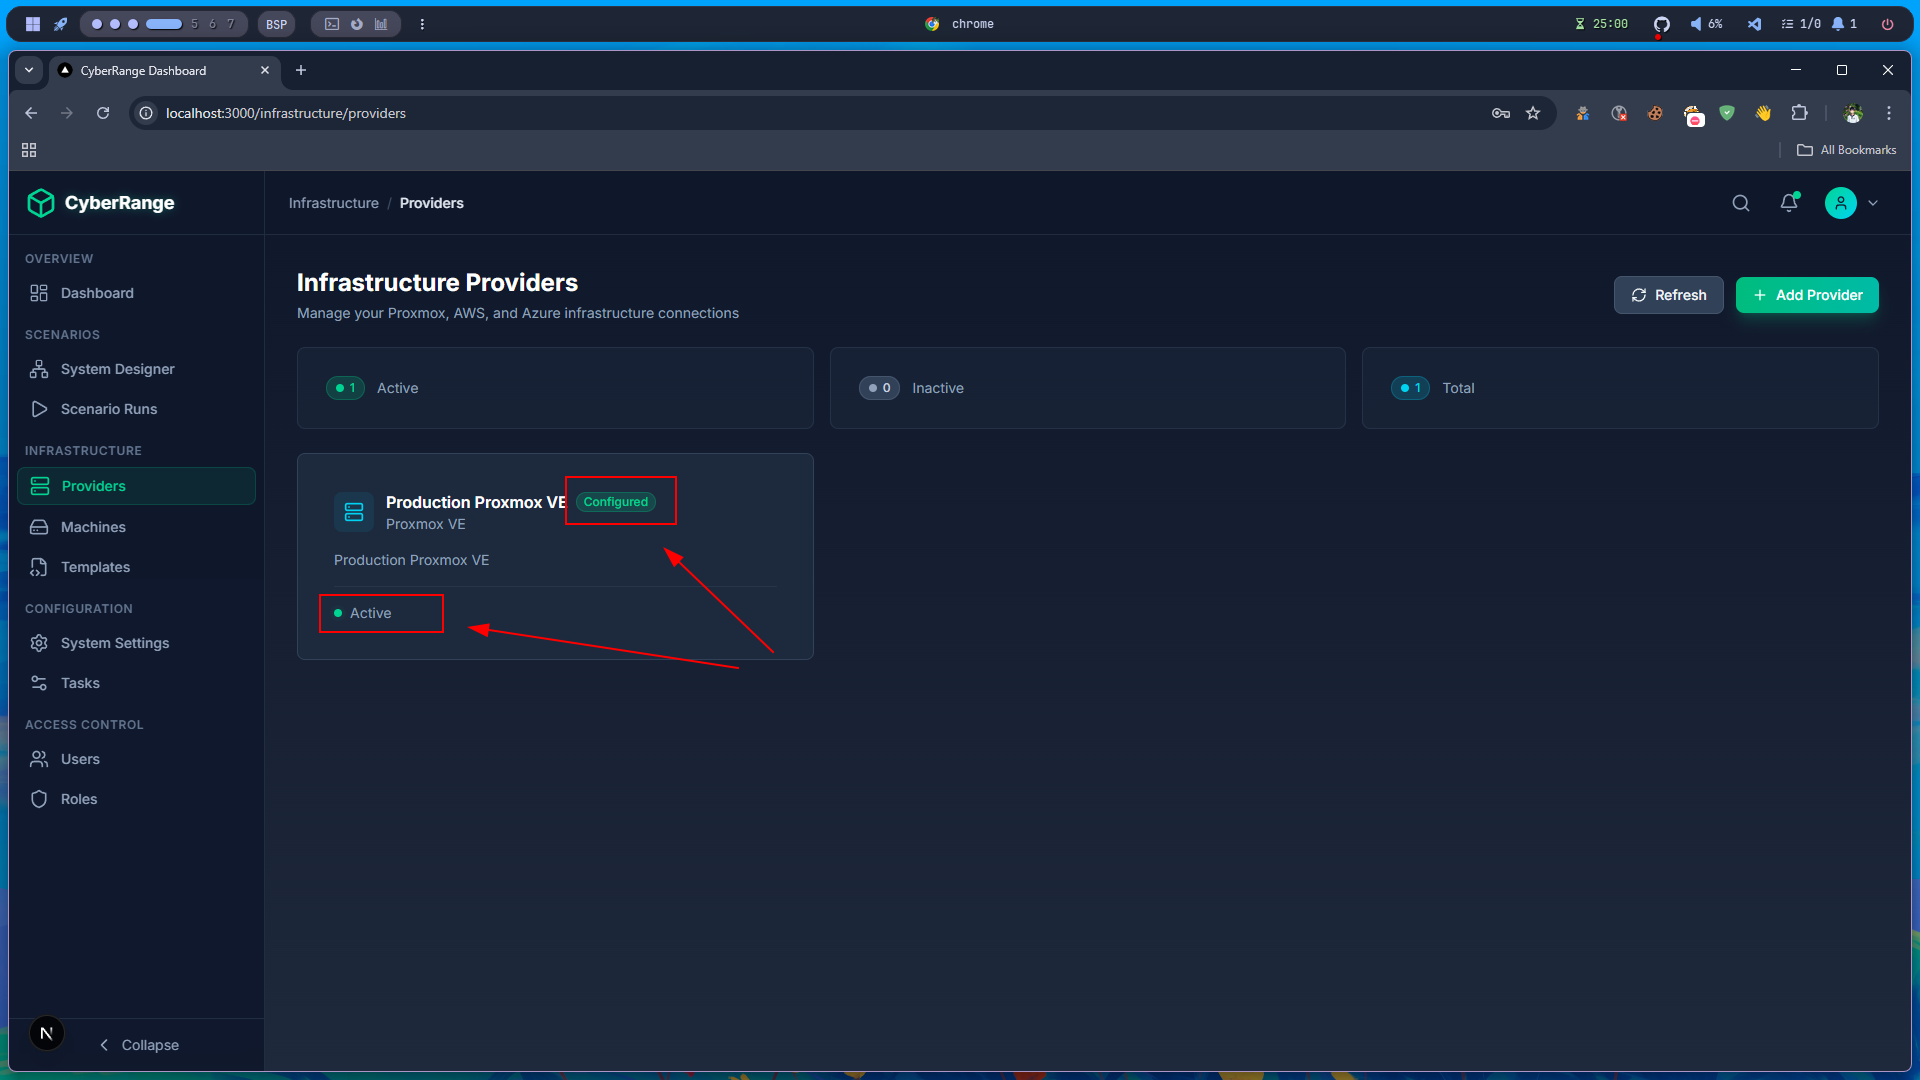
\includegraphics[width=0.95\textwidth]{images/infra/10.png}
    \caption{Configured provider state.}
    \label{fig:infra-provider-configured}
\end{figure}

\subsection{Phase 2: Template and Resource Preparation}
The objective of this phase was to prepare reusable deployment artifacts and resource definitions that support repeatable scenario instantiation. Core functions included template registration, metadata organization, resource mapping, machine synchronization, and readiness validation for deployment reuse.

This phase contributes implementation stability by reducing manual provisioning variance. Reusable templates ensure that scenario runs are created from consistent baselines, which improves reproducibility and simplifies troubleshooting. In the implemented platform, this phase is supported by both the infrastructure-side Proxmox inventory and the dashboard-side template and machine management views.

The operational workflow for template and resource preparation is as follows:

\begin{enumerate}
    \item Verify that the Proxmox node already contains the required base machines, network segments, and storage resources for cyber-range provisioning.
    \item Open \texttt{Infrastructure $\rightarrow$ Templates} to register or refresh reusable Packer templates from source repositories.
    \item Validate template status so only ready-to-use images are exposed to later scenario design and deployment workflows.
    \item Open \texttt{Infrastructure $\rightarrow$ Machines} to synchronize provisioned VMs/LXC resources and confirm runtime status, node placement, and resource allocation.
    \item Reuse these prepared templates and synchronized machines as stable infrastructure inputs for scenario instantiation.
\end{enumerate}

\begin{figure}[H]
    \centering
    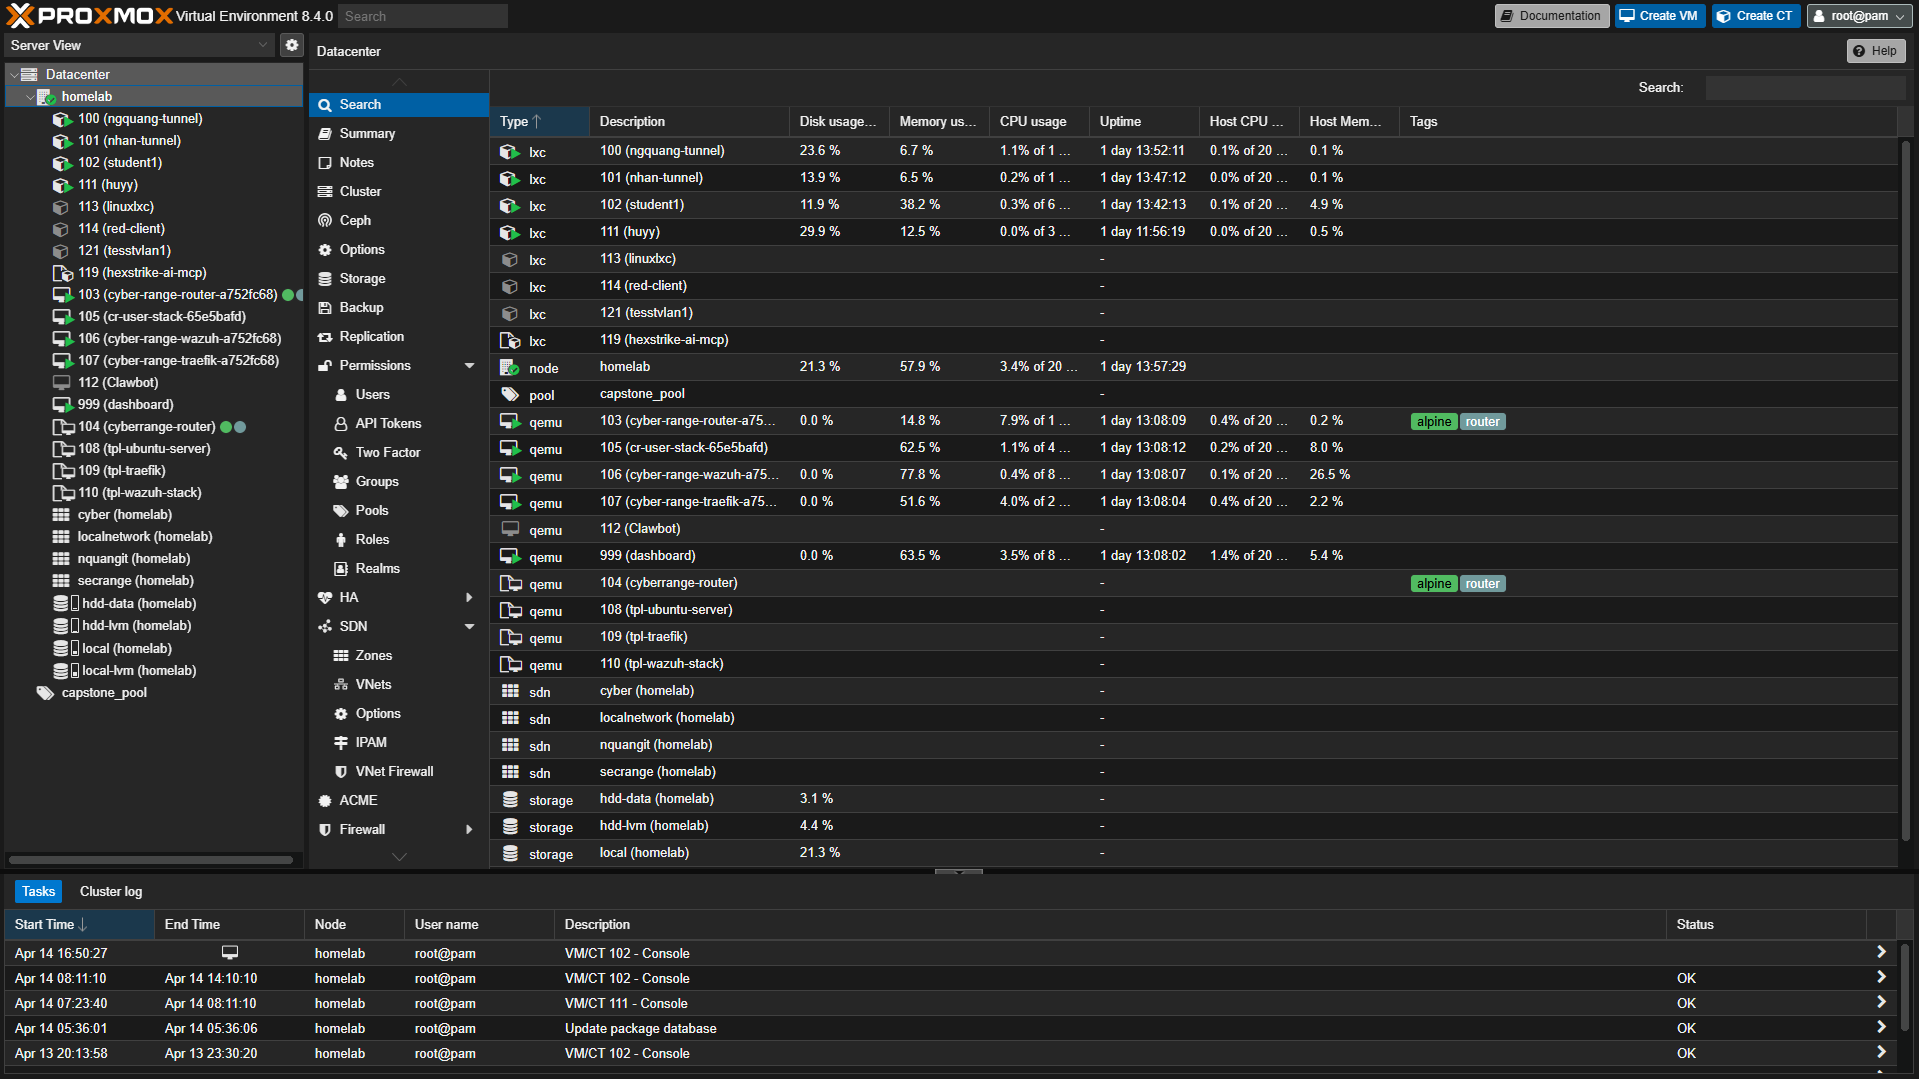
\includegraphics[width=0.95\textwidth]{images/wweb/promox.png}
    \caption{Proxmox inventory view.}
    \label{fig:phase2-proxmox-inventory}
\end{figure}

\begin{figure}[H]
    \centering
    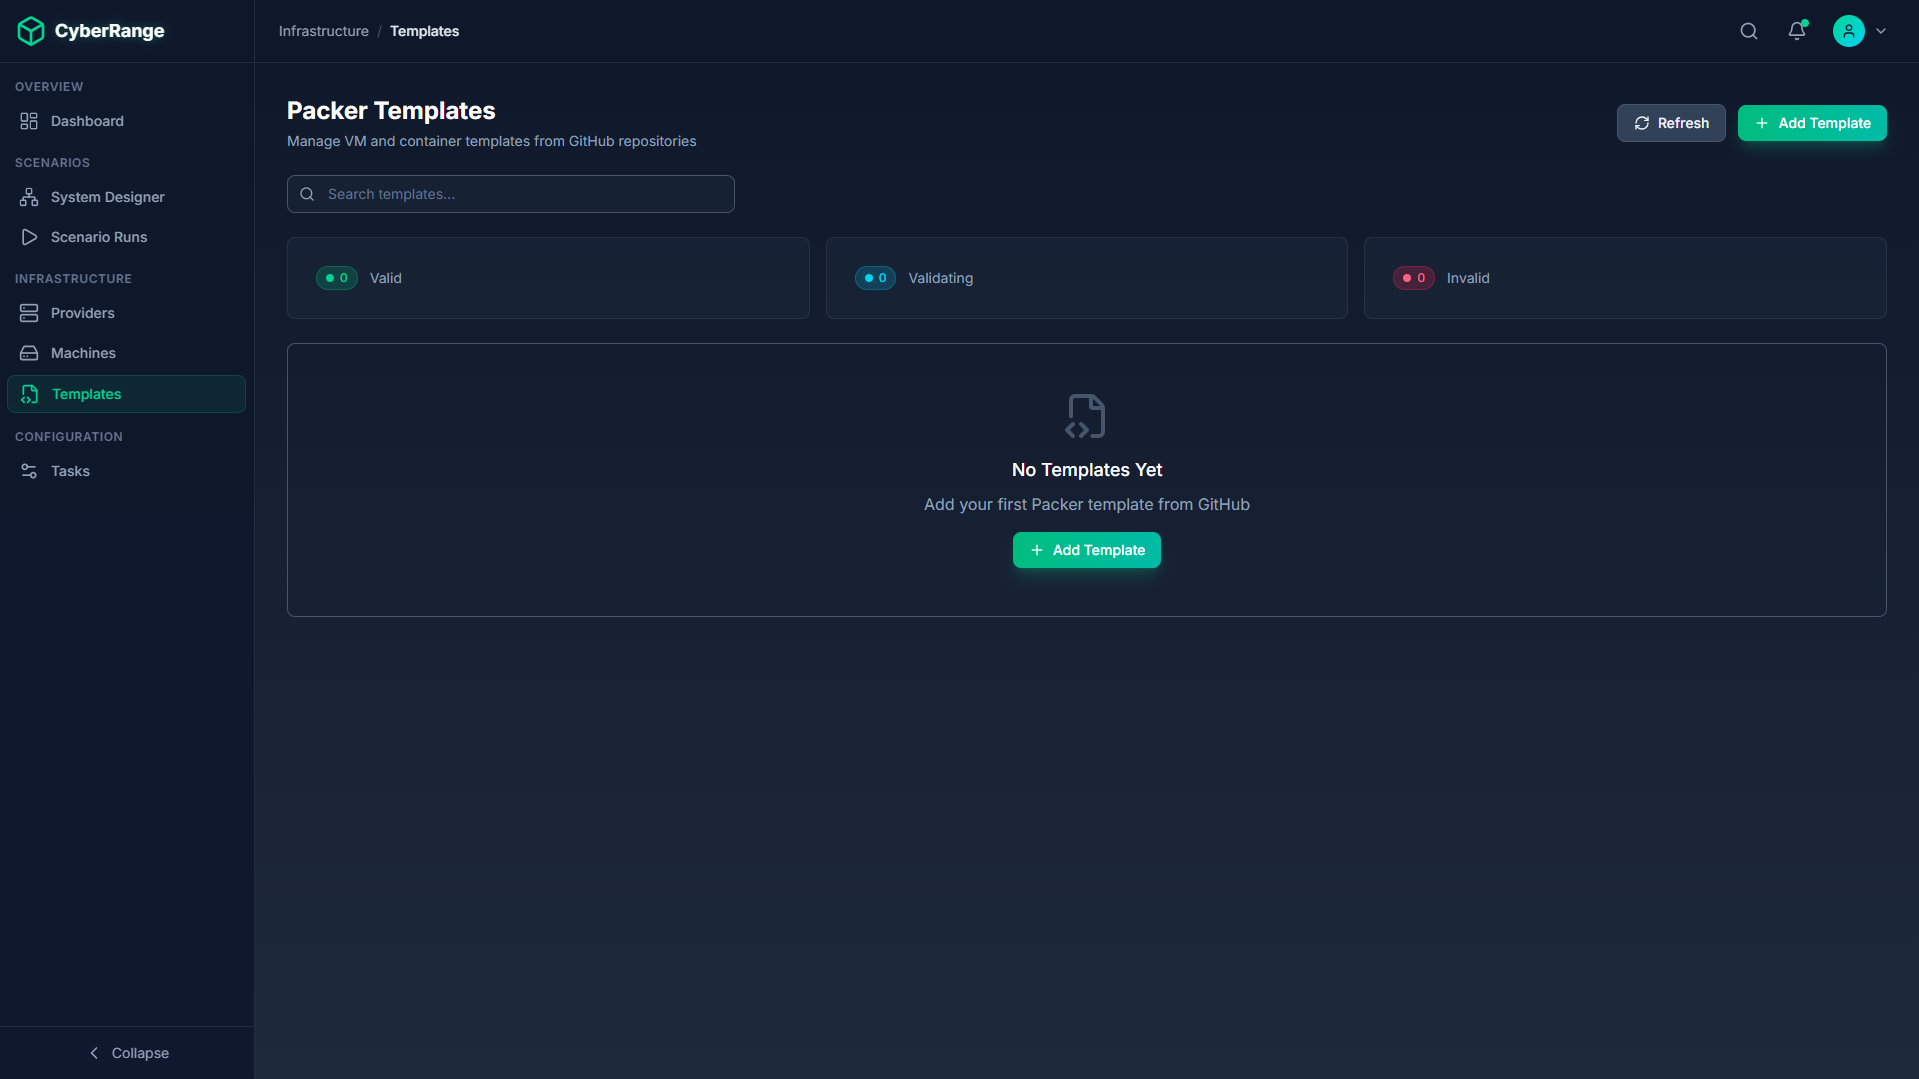
\includegraphics[width=0.95\textwidth]{images/wweb/template.png}
    \caption{Packer template management.}
    \label{fig:phase2-template-management}
\end{figure}

\begin{figure}[H]
    \centering
    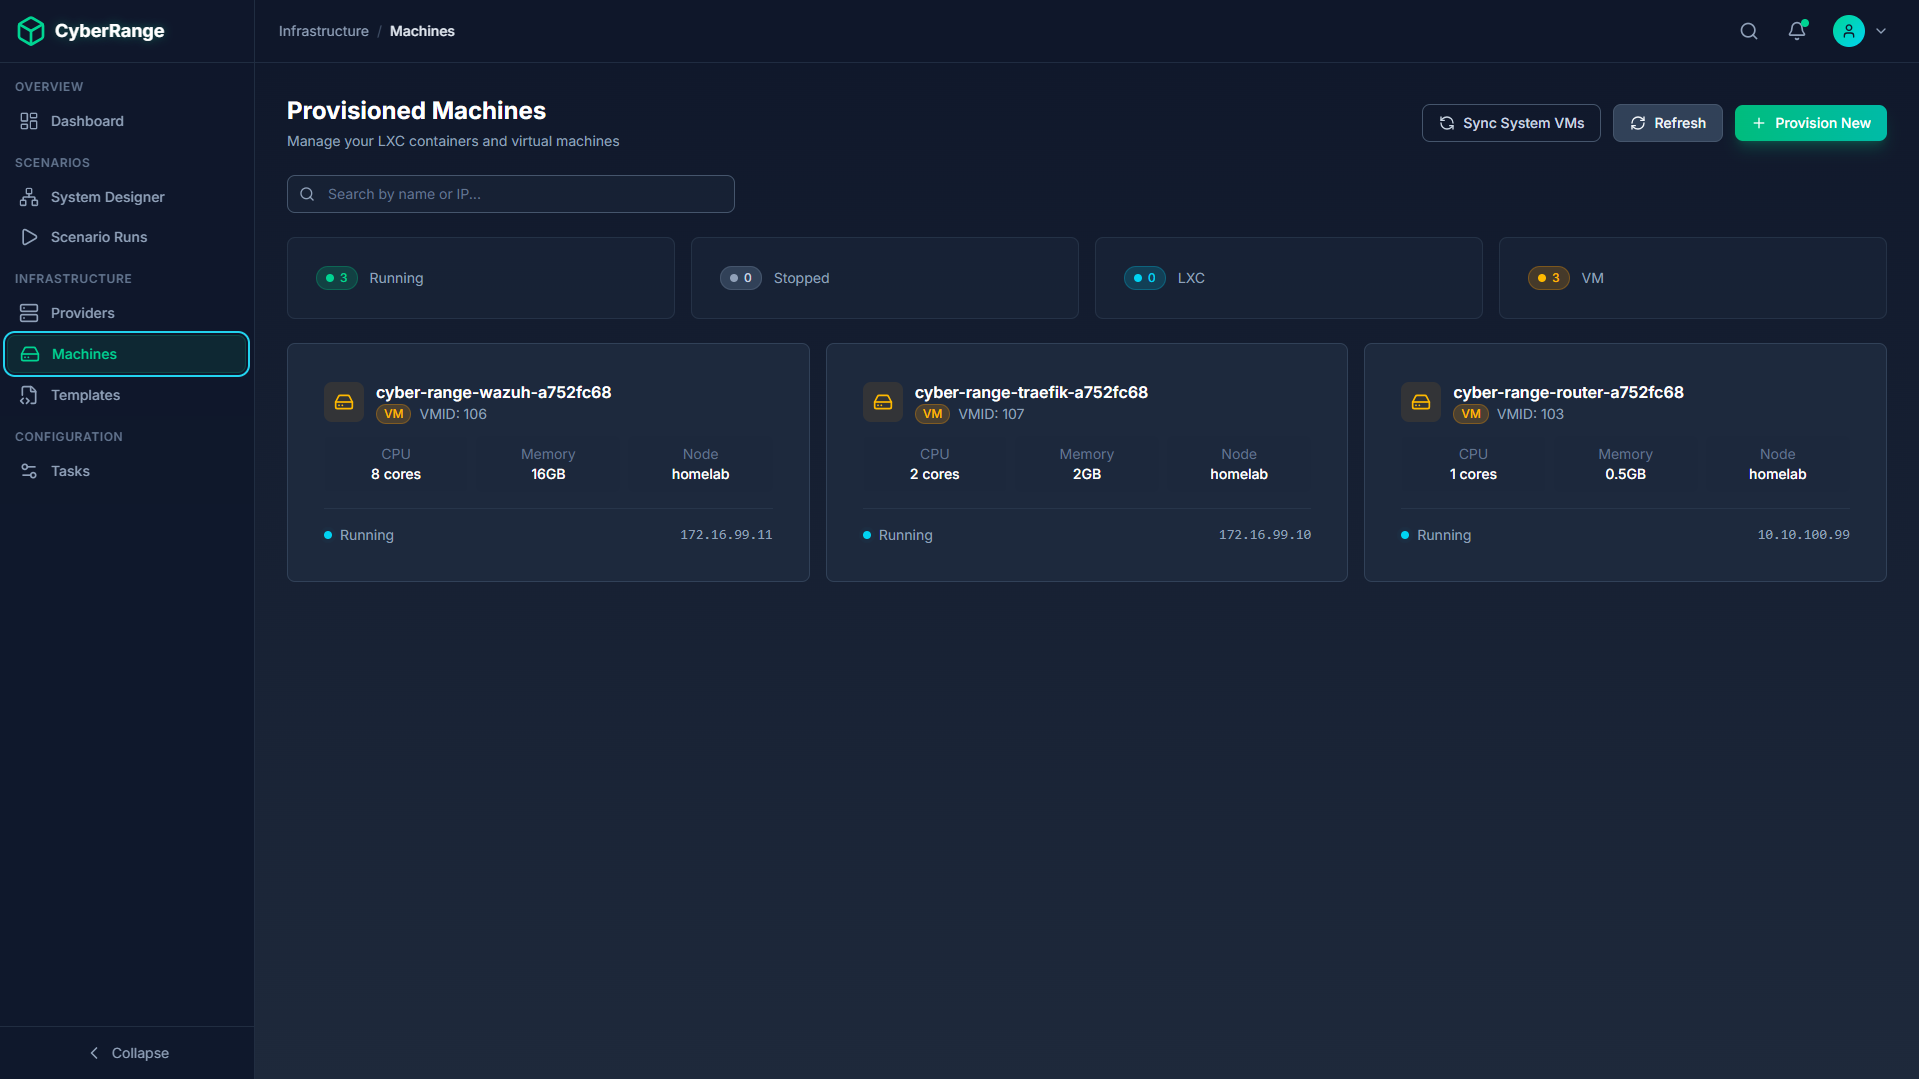
\includegraphics[width=0.95\textwidth]{images/wweb/machine.png}
    \caption{Provisioned machine view.}
    \label{fig:phase2-machine-management}
\end{figure}

\subsection{Phase 3: Scenario Definition and Management}
The objective of this phase was to formalize executable training logic through scenario entities. Core functions included scenario creation, update and version control, linkage to provider/template assets, and lifecycle state management.

This phase bridges static infrastructure preparation and dynamic execution. By encapsulating deployment logic into scenario definitions, the platform enables controlled and repeatable training workflows through the dashboard.

The scenario authoring workflow is captured in \texttt{images/scenarios}. The validated sequence used in implementation is:

\begin{enumerate}
    \item Open \texttt{Scenarios $\rightarrow$ System Designer}, then select \texttt{New Scenario}.
    \item Enter scenario name and description, then bind the scenario to a configured infrastructure provider.
    \item Use the visual editor to drag and place runtime components into the user stack topology.
    \item Configure node-level parameters on the right panel (for example API key bindings for Blue Team/Red Team agents).
    \item For custom application containers, select Docker Compose mode, provide repository and branch, verify compose metadata, and map exposed ports.
    \item Save scenario changes before triggering deployment.
\end{enumerate}

In the implemented system, the platform provides three ready-made scenarios so that instructors or learners can launch training environments without designing the topology from scratch. The first is a \textit{Red Team Single} scenario, in which the learner is provided with a dedicated WAF interface, a Red Team attack workspace, and a vulnerable target web application. This scenario is designed for offensive practice and includes AI-assisted support to help interpret attack attempts and request behavior.

The second is a \textit{Blue Team Single} scenario, in which the learner is provided with a WAF layer together with a Blue Team analysis interface for log inspection, alert review, and AI-assisted interpretation. In the current implementation, this defensive workspace is delivered through the BlueAgent WAF Console presented later in this chapter. This scenario emphasizes defensive analysis, allowing trainees to focus on monitoring evidence and understanding how suspicious requests are detected and explained.

The third is a \textit{Dual} scenario, which combines both operational perspectives into one linked environment. In this mode, the Red Team attacks the target web application while the resulting traffic and security events are forwarded to the Blue Team workspace for investigation. This linkage creates a more realistic end-to-end cyber range exercise in which offensive actions produce defensive telemetry that can be reviewed in near real time.

To support these scenarios, the project includes a vulnerable SQL-focused target application used as an attack surface during training. This target application is paired with the Red Team workspace in offensive exercises and becomes the common event source for the linked dual scenario.

\begin{figure}[H]
    \centering
    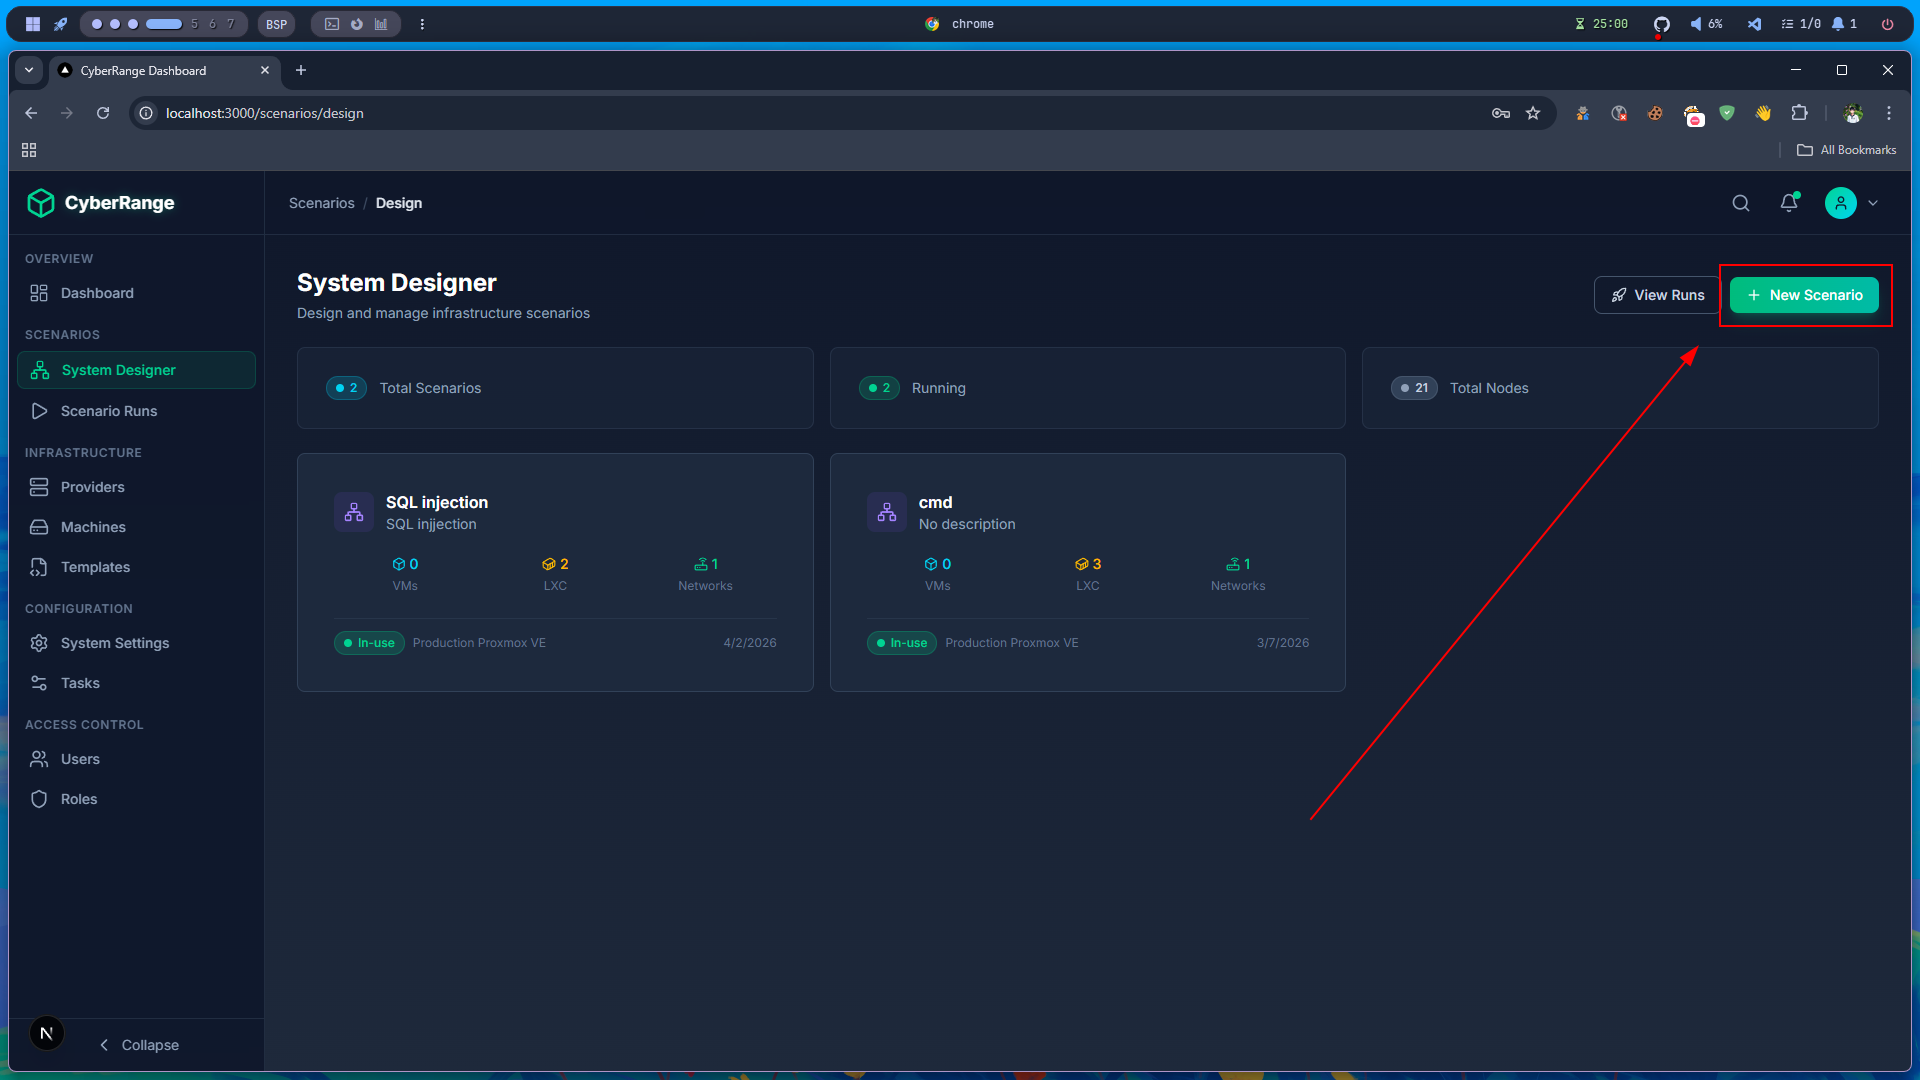
\includegraphics[width=0.95\textwidth]{images/scenarios/1.png}
    \caption{System Designer overview.}
    \label{fig:scenario-designer-entry}
\end{figure}

\begin{figure}[H]
    \centering
    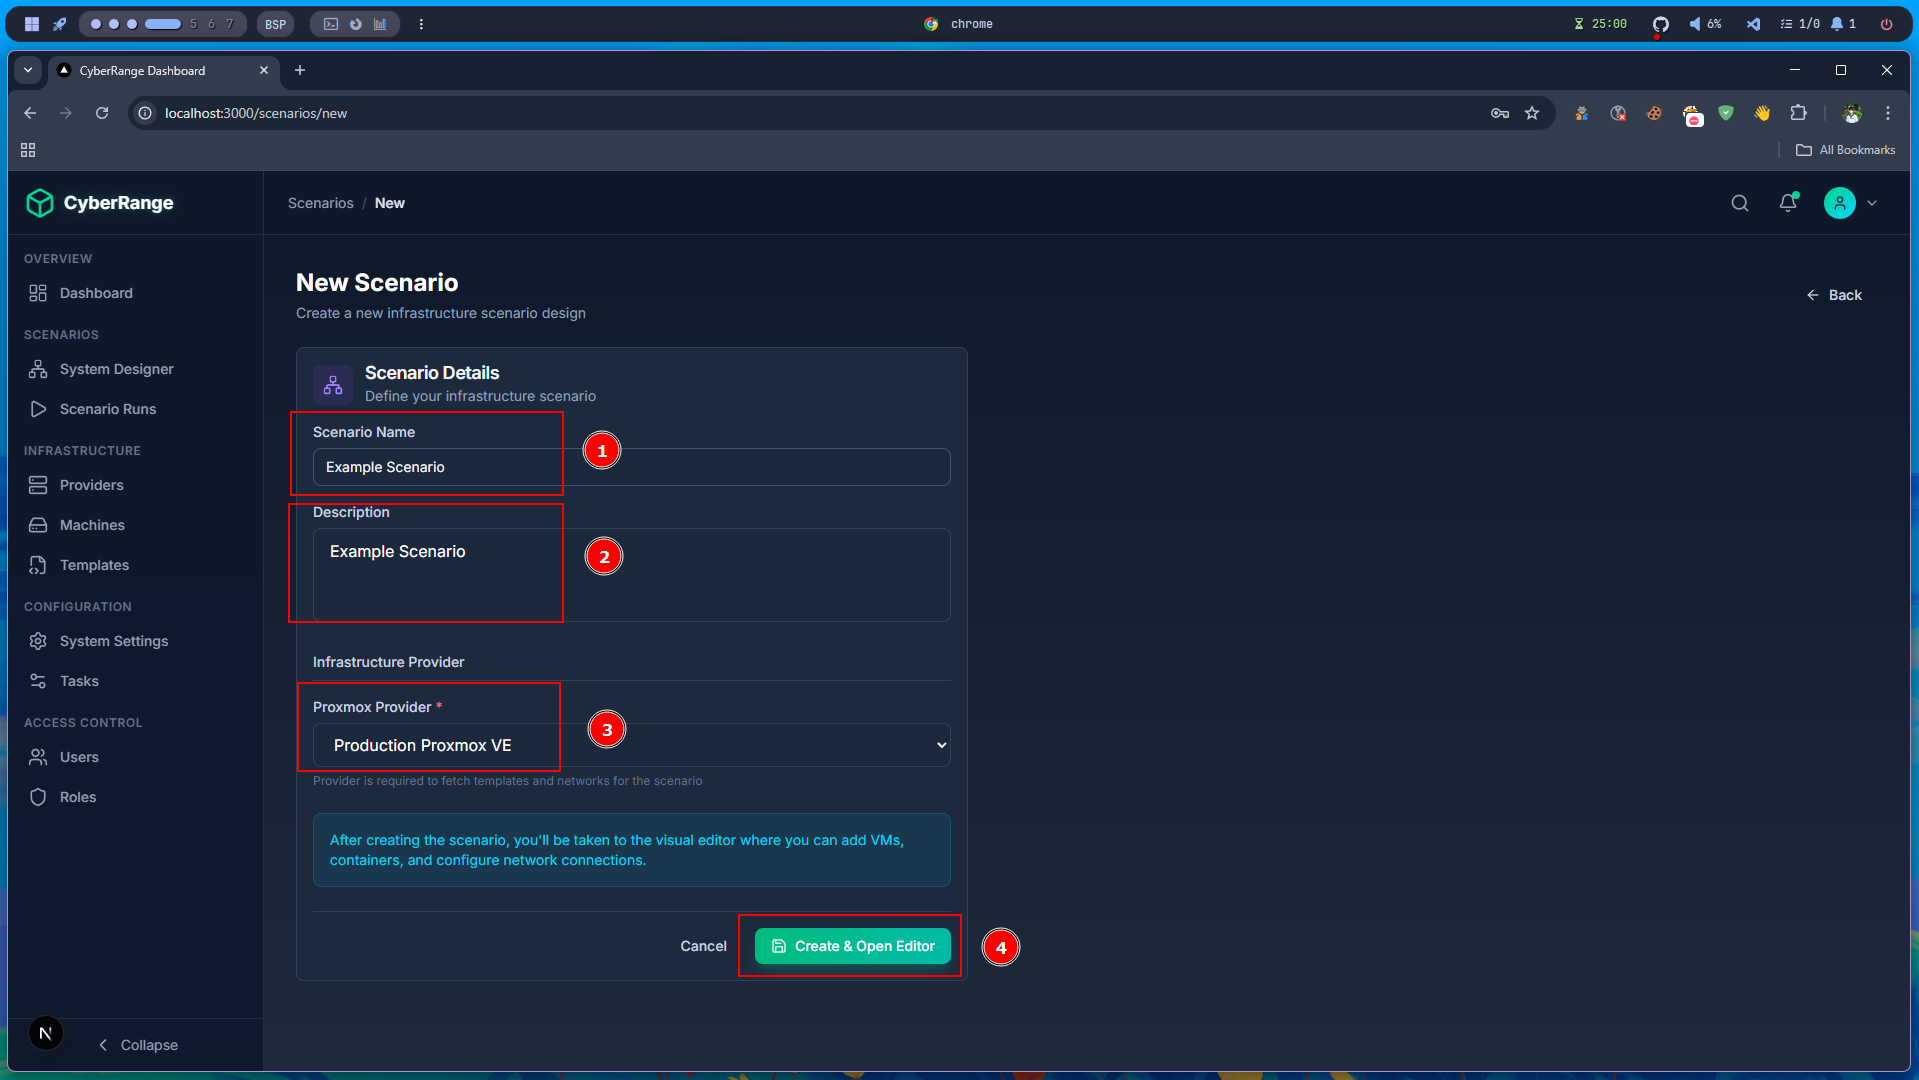
\includegraphics[width=0.95\textwidth]{images/scenarios/2.png}
    \caption{Scenario creation form.}
    \label{fig:scenario-create-form}
\end{figure}

\begin{figure}[H]
    \centering
    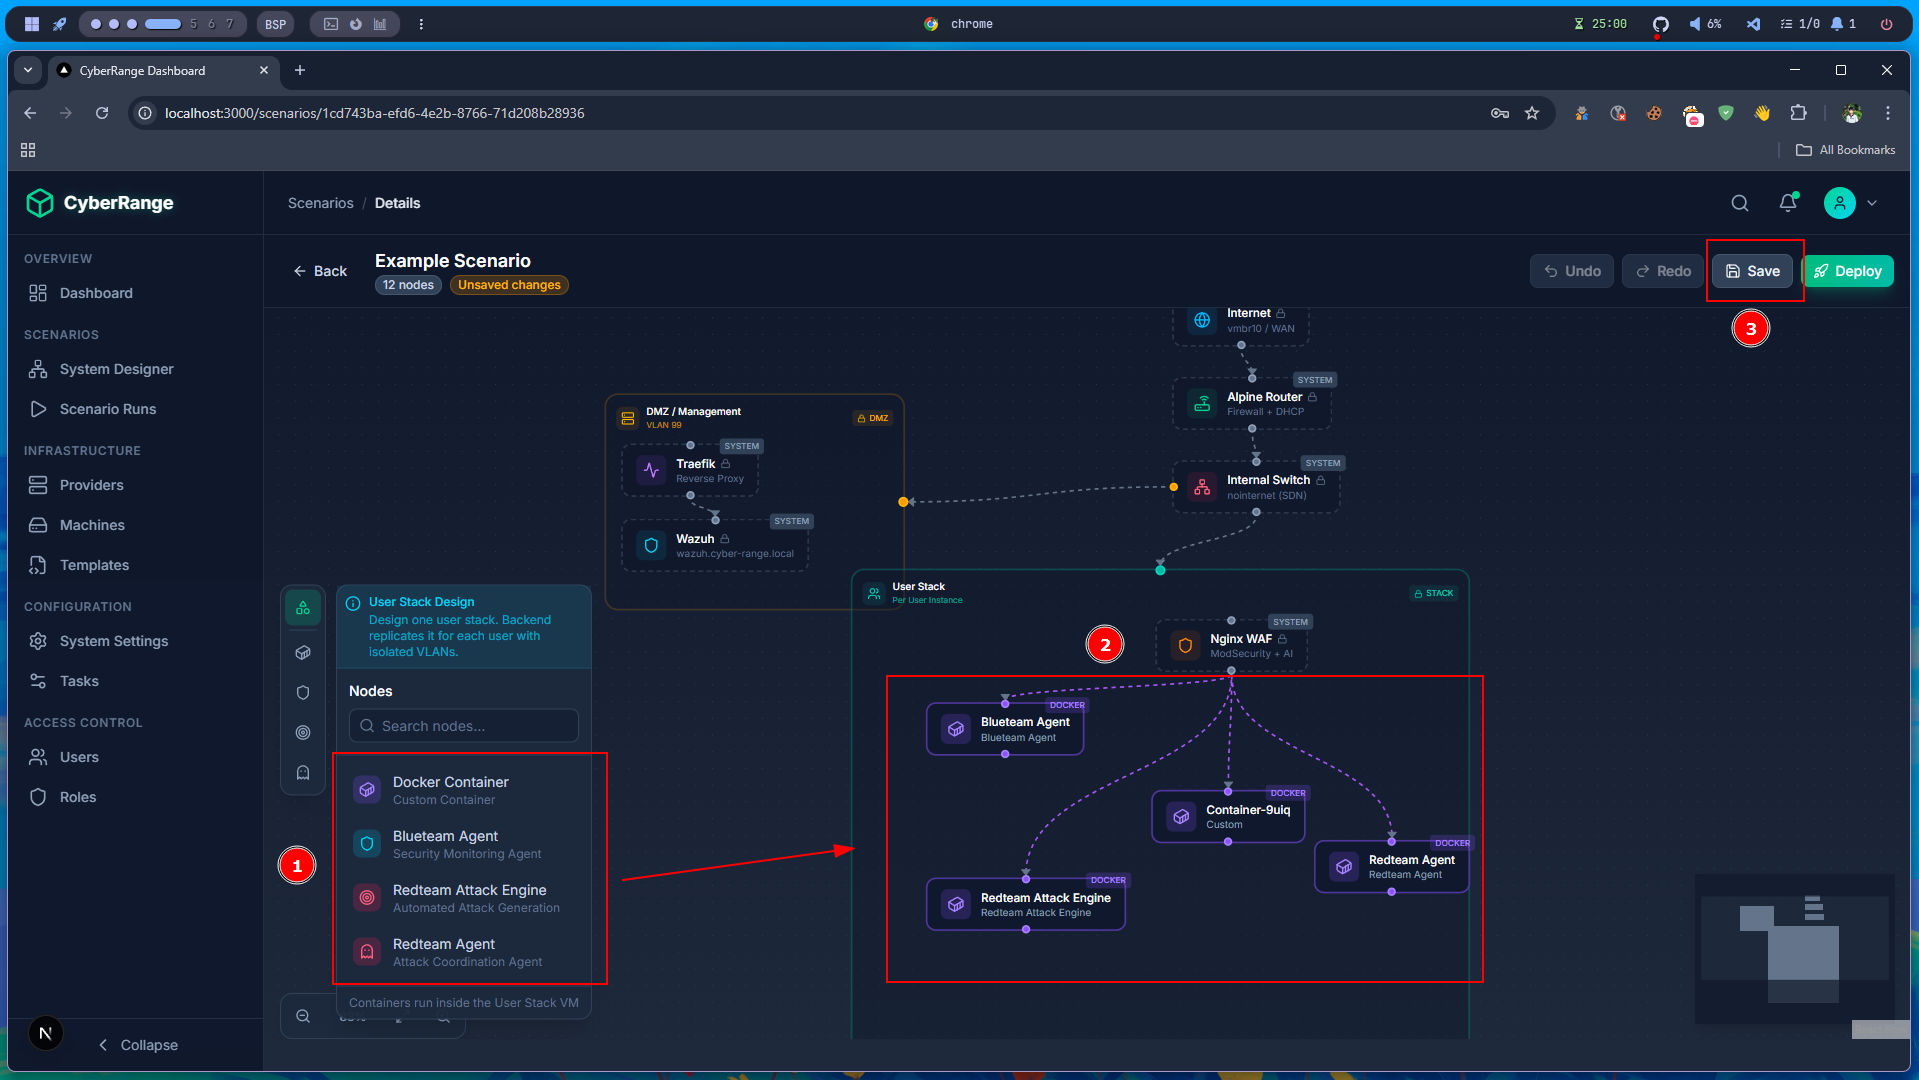
\includegraphics[width=0.95\textwidth]{images/scenarios/3.png}
    \caption{Scenario topology editor.}
    \label{fig:scenario-visual-editor}
\end{figure}

\begin{figure}[H]
    \centering
    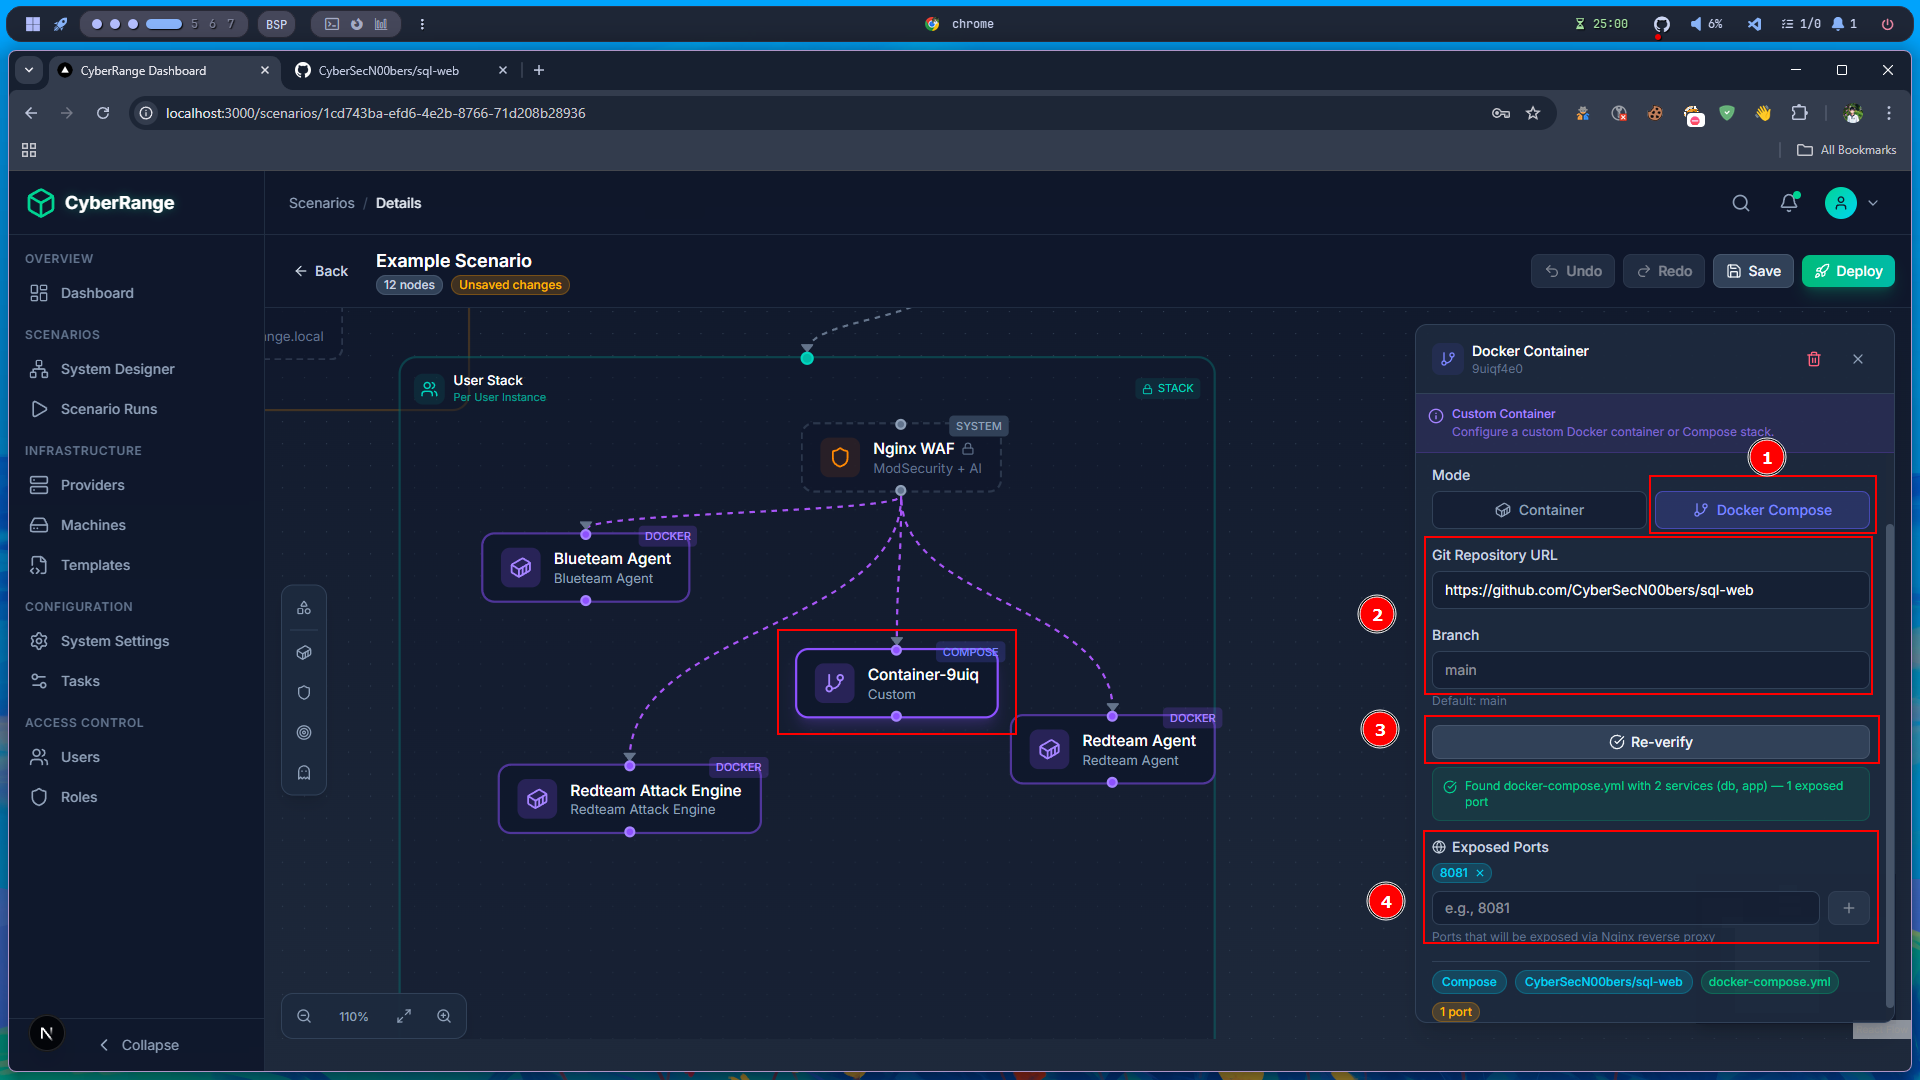
\includegraphics[width=0.95\textwidth]{images/scenarios/5.png}
    \caption{Custom container configuration.}
    \label{fig:scenario-docker-compose-config}
\end{figure}

\begin{figure}[H]
    \centering
    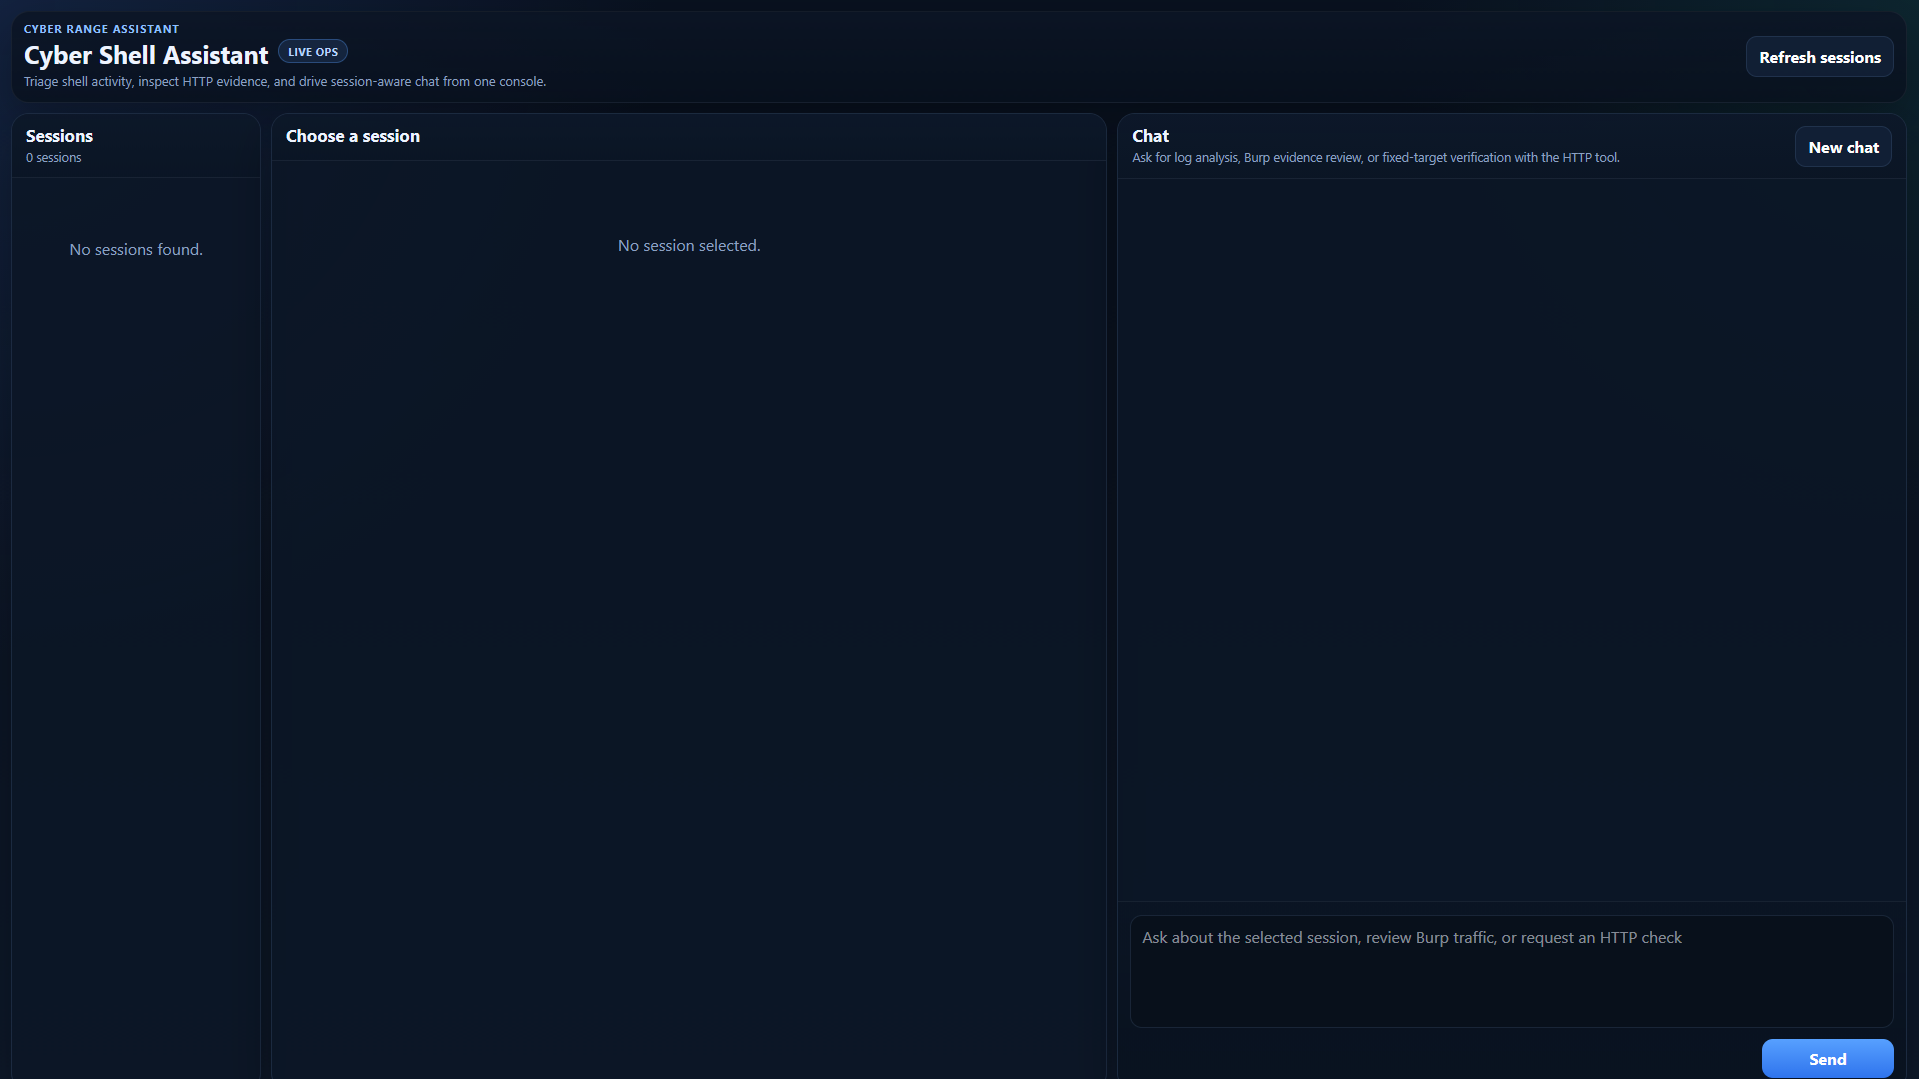
\includegraphics[width=0.95\textwidth]{images/wweb/redtam agent.png}
    \caption{Red Team single-scenario workspace with AI-assisted attack support.}
    \label{fig:scenario-redteam-workspace}
\end{figure}

\begin{figure}[H]
    \centering
    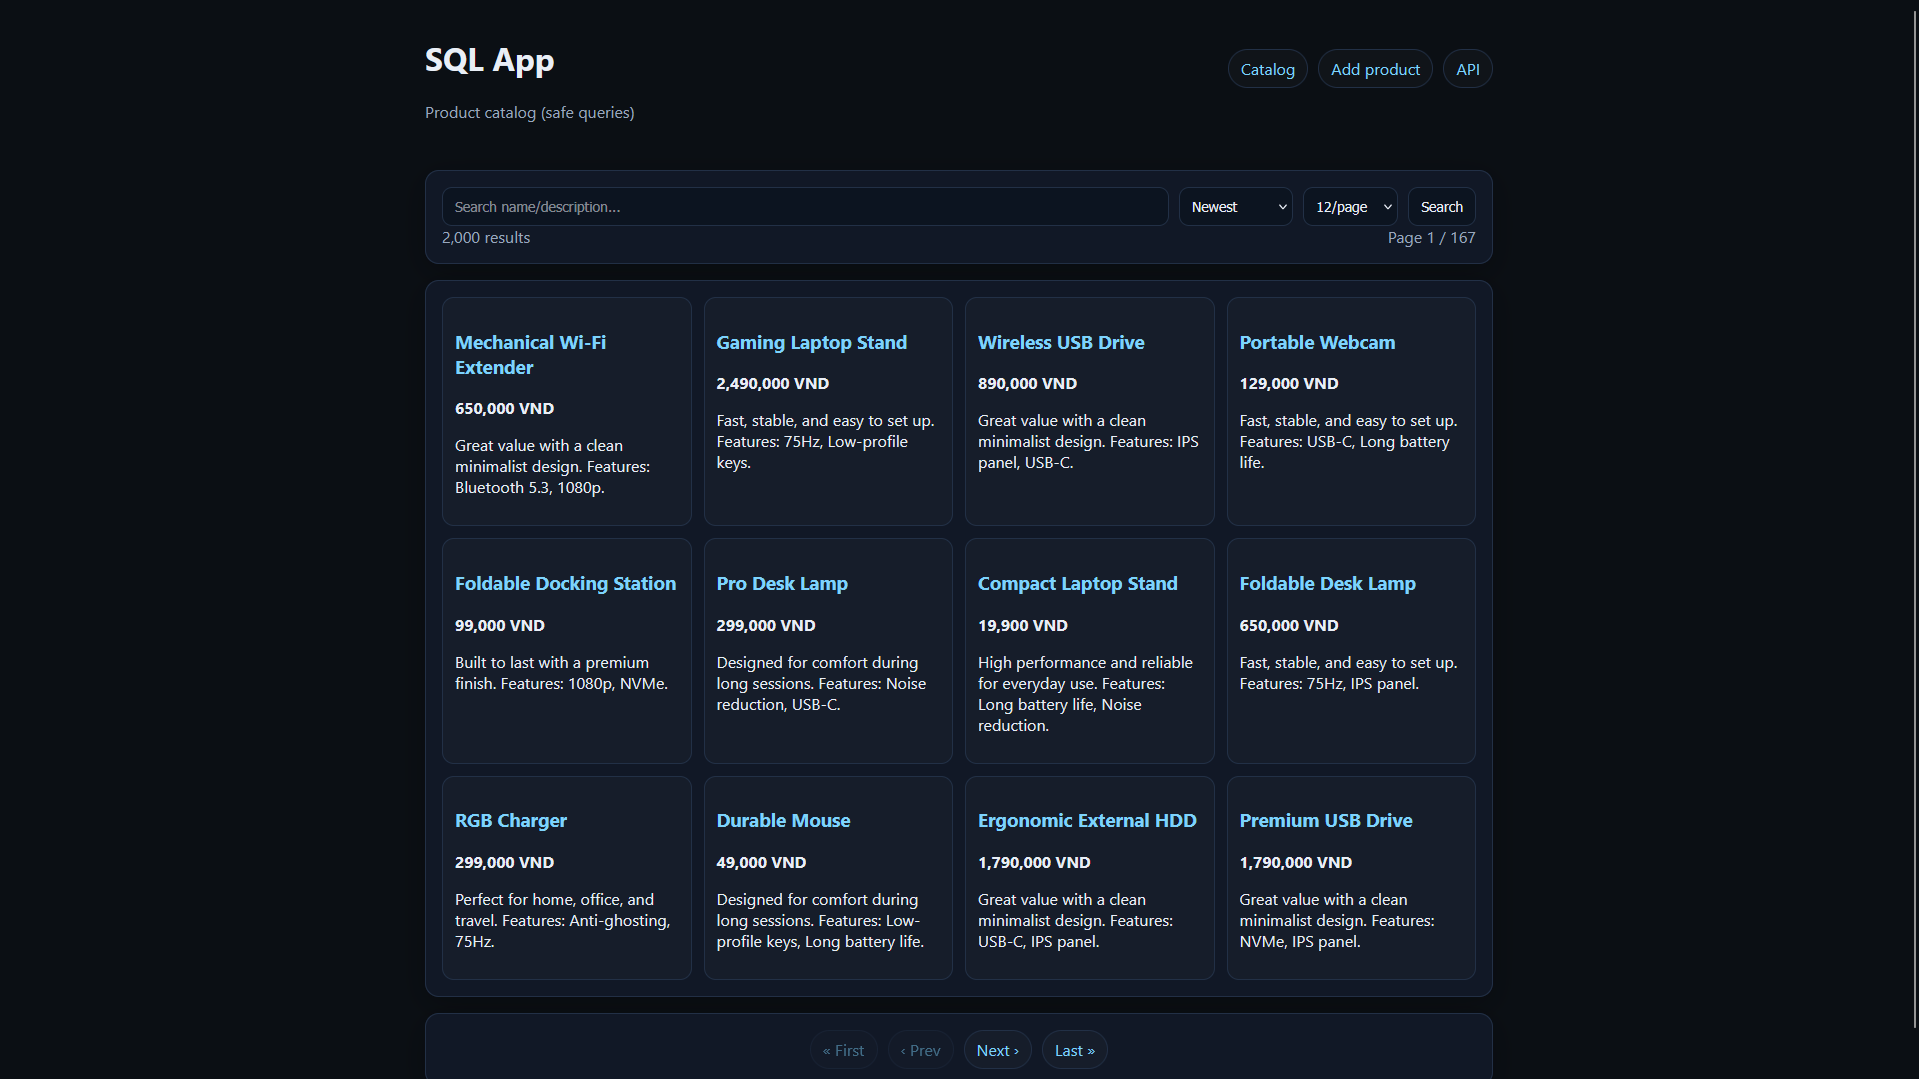
\includegraphics[width=0.95\textwidth]{images/wweb/sqlapp.png}
    \caption{Vulnerable SQL target web application used in predefined scenarios.}
    \label{fig:scenario-sqlapp-target}
\end{figure}

\subsection{Phase 4: Scenario Deployment and Execution}
The objective of this phase was to execute scenario provisioning through asynchronous orchestration. Core functions included deployment triggering, job dispatch, runtime state transitions, and execution feedback propagation to dashboard views.

This phase is operationally central because it transforms configuration artifacts into active training environments. Asynchronous execution is essential here because deployment operations are long-running and cannot block dashboard responsiveness.

The deployment and post-deployment access workflow is documented in \path{images/scenarios/deploy}. The operational steps are:

\begin{enumerate}
    \item From \texttt{System Designer}, open scenario actions and select \texttt{Deploy}.
    \item Move to \texttt{Scenario Runs} to monitor state transitions (pending/running/failed/destroyed).
    \item Open run actions and select \texttt{View Resources} to inspect provisioned assets.
    \item Validate generated domains, runtime applications, and user stack health in the run access page.
    \item Open \texttt{Credentials} to retrieve access details (SSH, service credentials, and generated secrets).
    \item When training is complete, execute \texttt{Destroy} from run actions to release allocated resources.
\end{enumerate}

\begin{figure}[H]
    \centering
    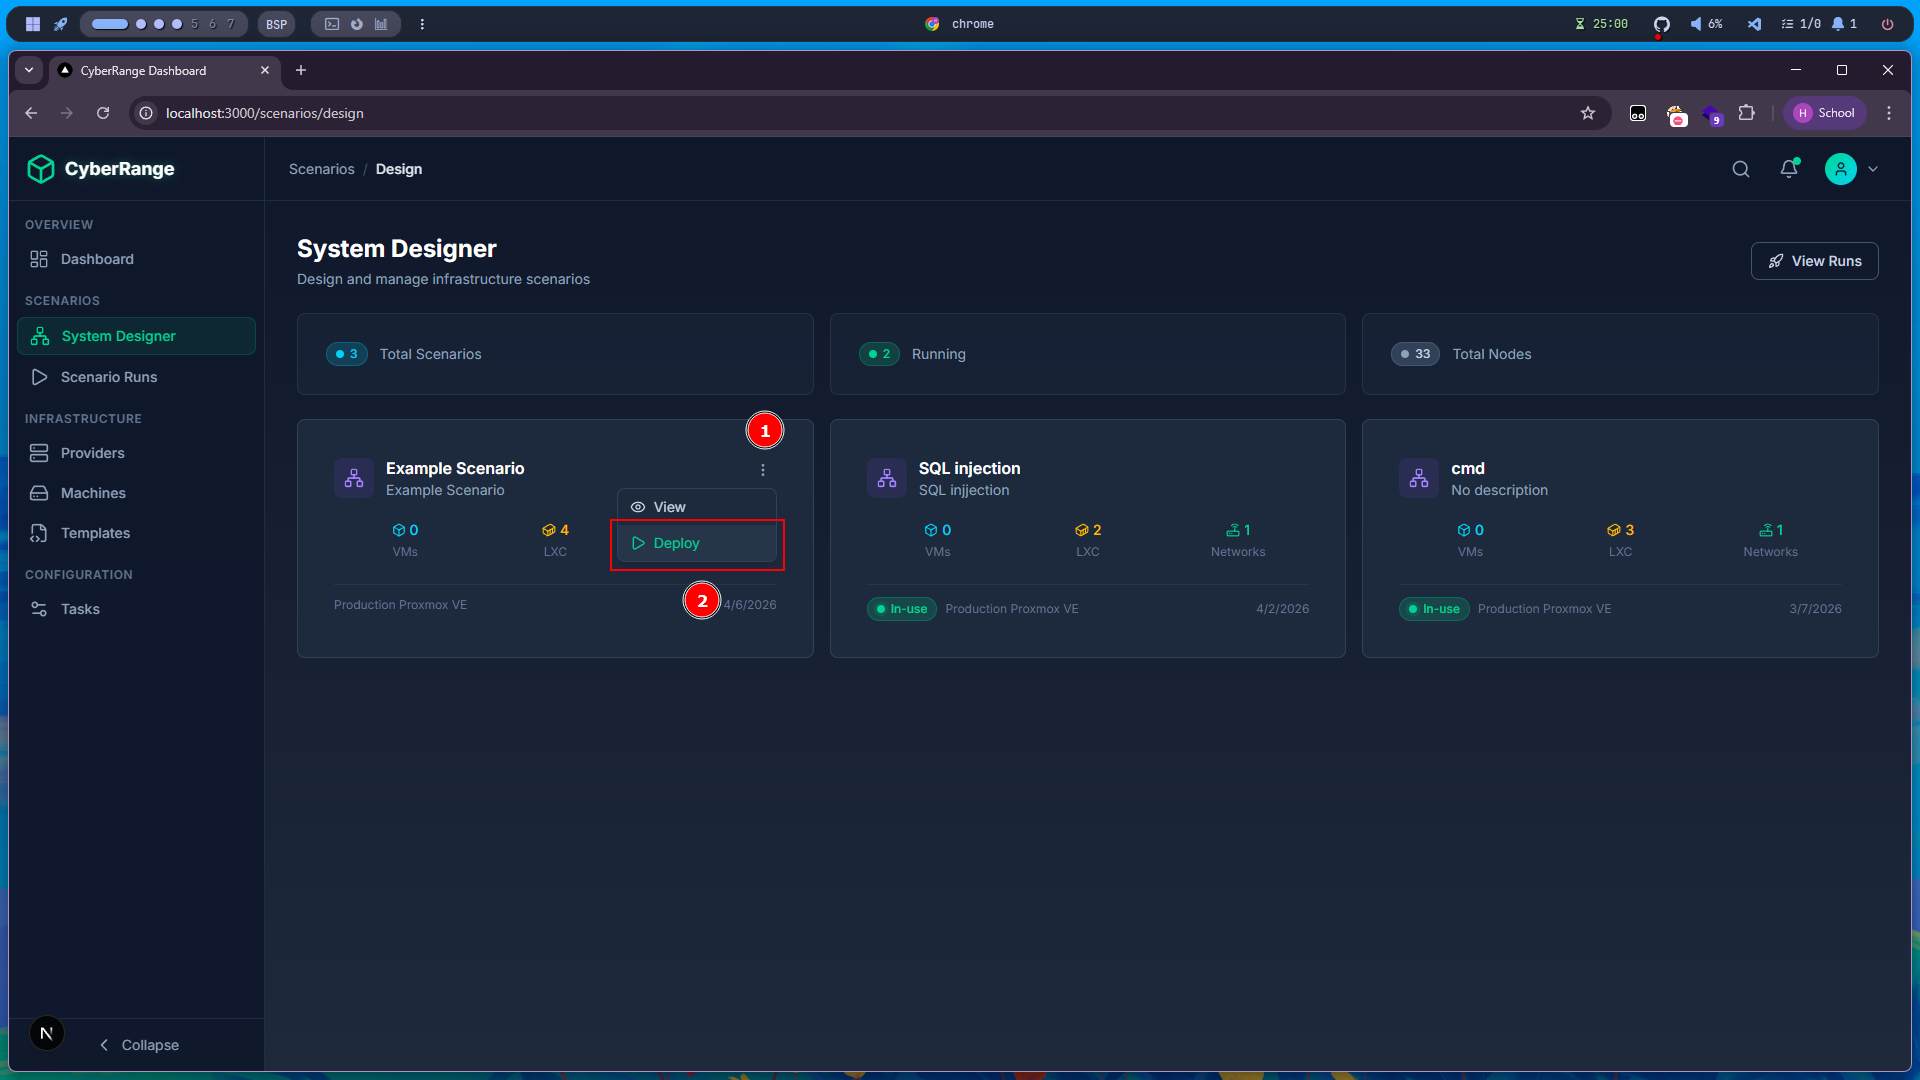
\includegraphics[width=0.95\textwidth]{images/scenarios/deploy/1.png}
    \caption{Scenario deploy action.}
    \label{fig:scenario-deploy-trigger}
\end{figure}

\begin{figure}[H]
    \centering
    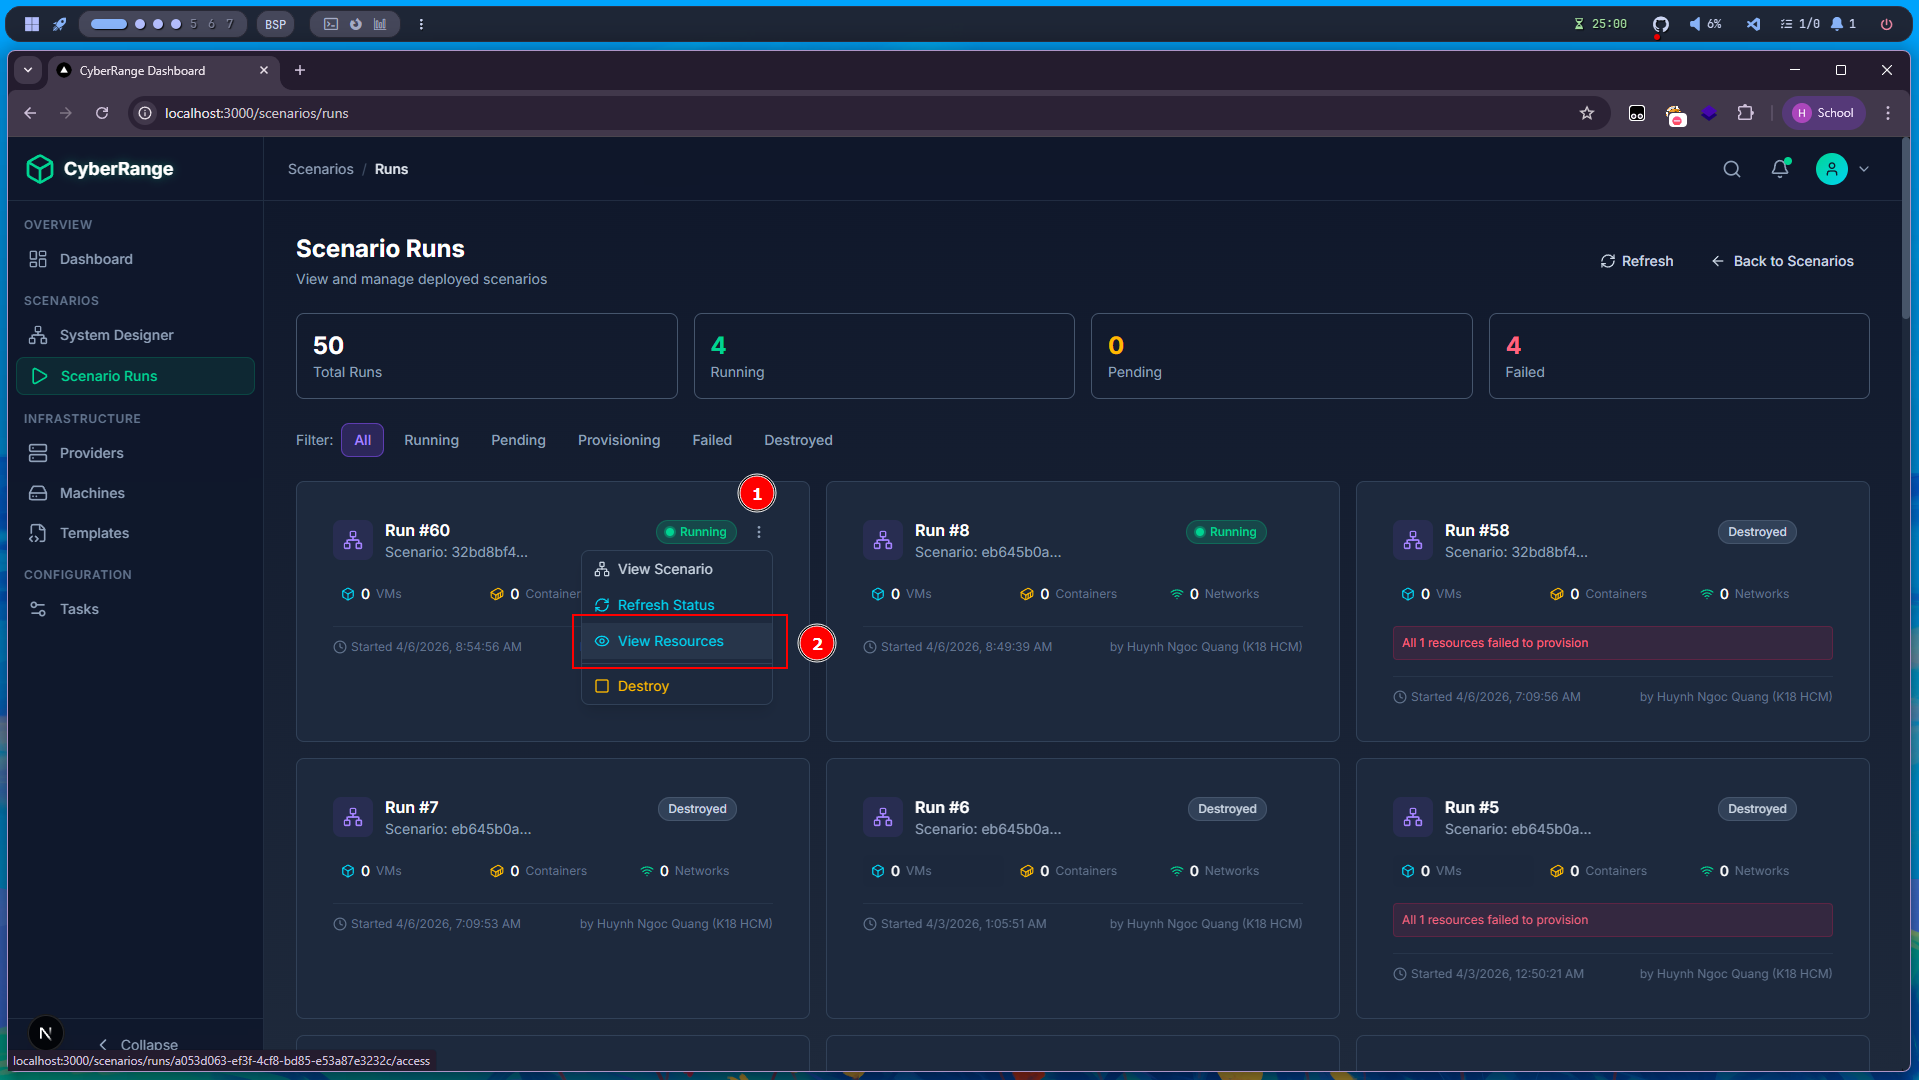
\includegraphics[width=0.95\textwidth]{images/scenarios/deploy/3.png}
    \caption{Run action menu.}
    \label{fig:scenario-run-view-resources}
\end{figure}

\begin{figure}[H]
    \centering
    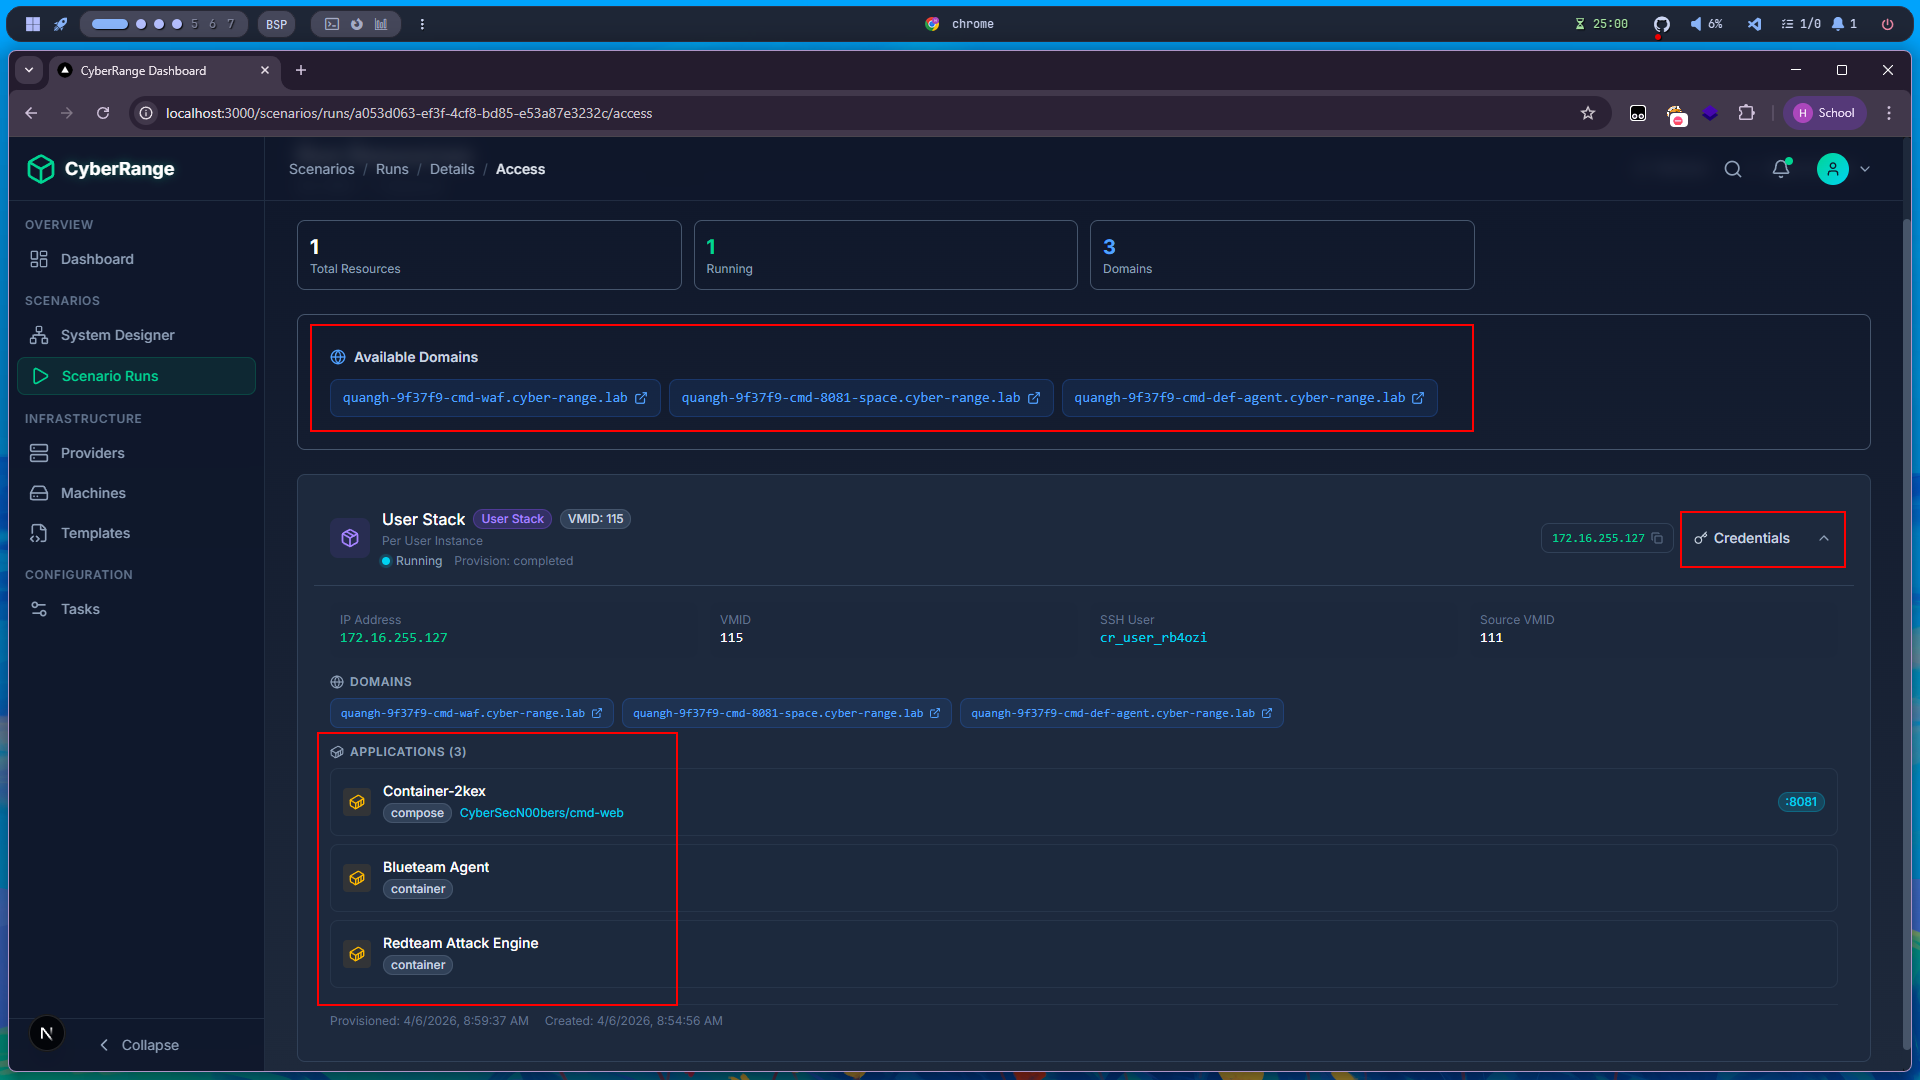
\includegraphics[width=0.95\textwidth]{images/scenarios/deploy/4.png}
    \caption{Run access view.}
    \label{fig:scenario-run-access-view}
\end{figure}

\begin{figure}[H]
    \centering
    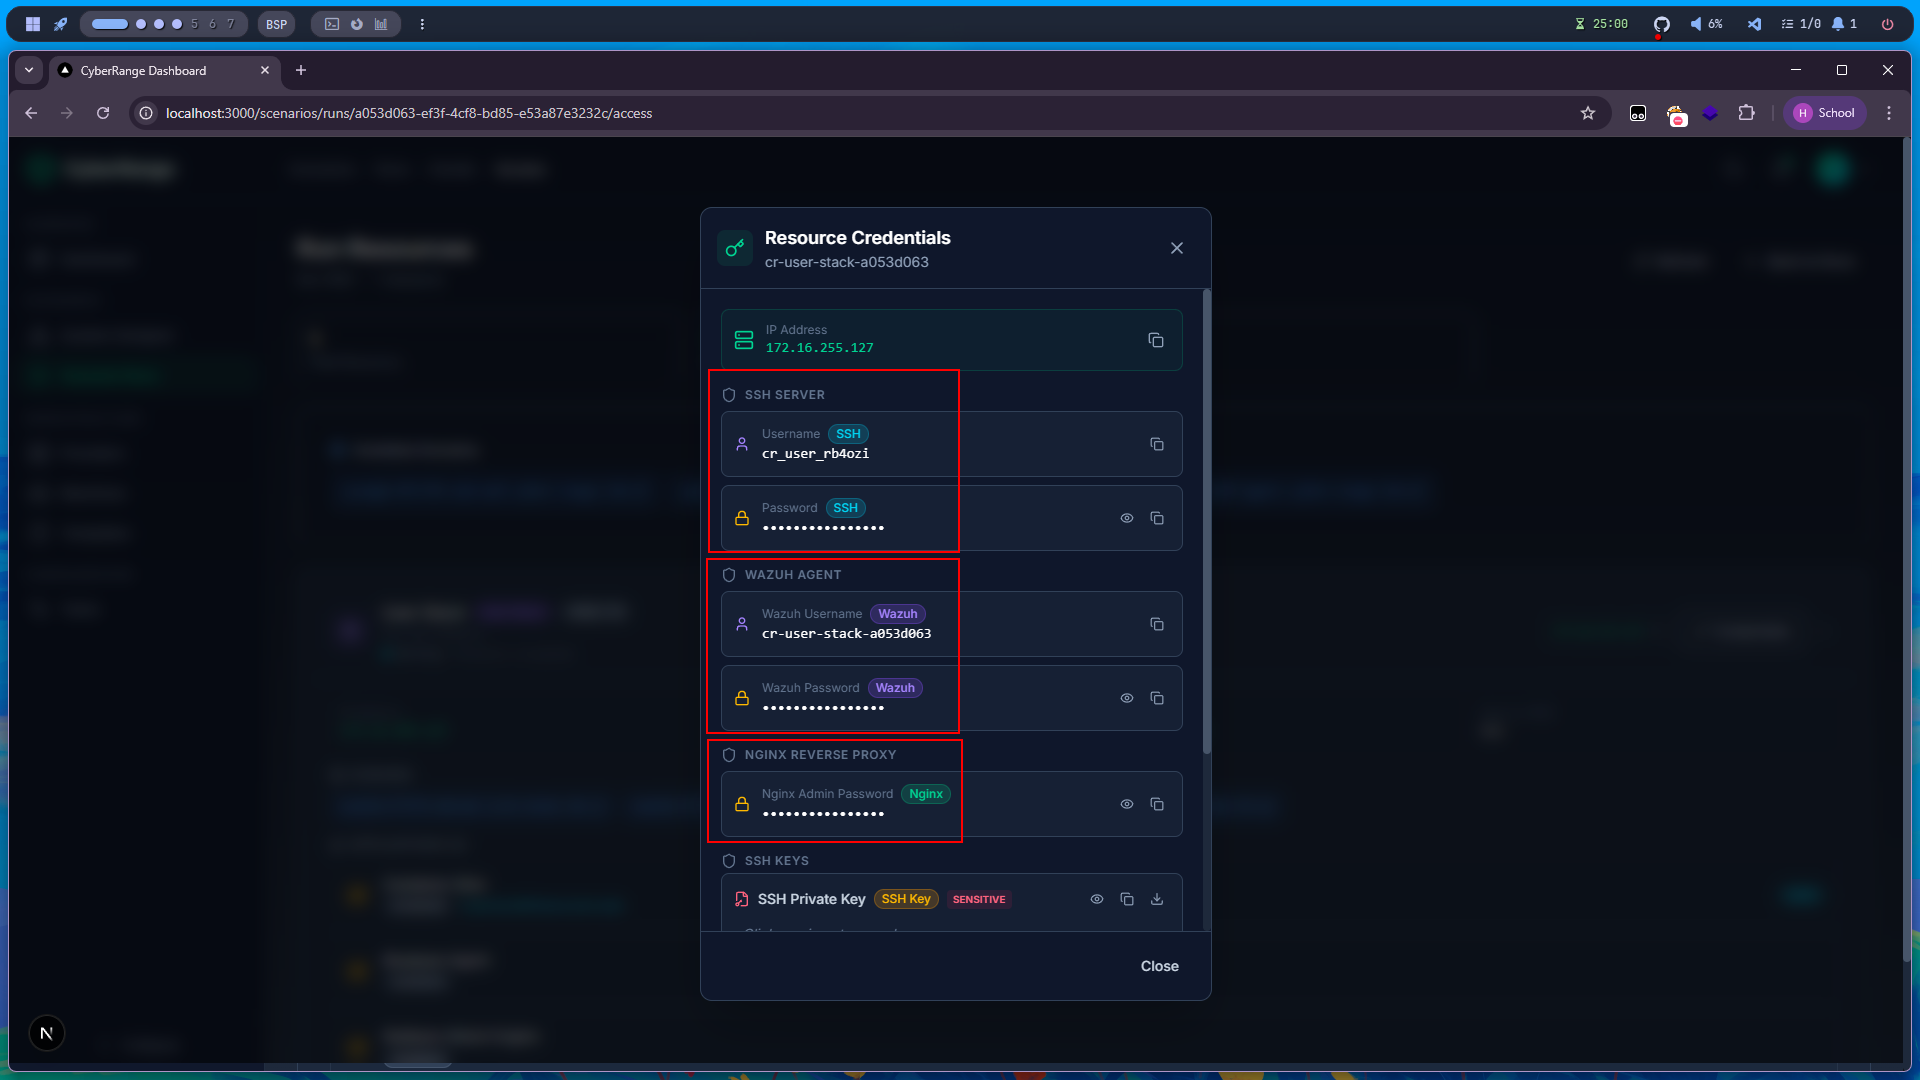
\includegraphics[width=0.95\textwidth]{images/scenarios/deploy/5.png}
    \caption{Resource credentials panel.}
    \label{fig:scenario-run-credentials}
\end{figure}

\subsection{Phase 5: Monitoring and Task Management}
The objective of this phase was to provide transparent execution observability for operators and evaluators. Core functions included task/job status tracking, log inspection, failure identification, and retry-oriented operational control.

This phase supports reliability and maintainability. By exposing execution traces and task states, it enables faster diagnosis of provisioning issues and improves confidence in repeated scenario runs. In the implemented dashboard, monitoring is not limited to SIEM review; it also includes a configuration-task layer that standardizes recurring machine automation steps such as Docker installation, SSH hardening, monitoring deployment, firewall setup, and reverse-proxy preparation.

The configuration-task workflow provides the following control benefits:

\begin{enumerate}
    \item Centralizing reusable automation tasks so administrators can apply consistent machine setup logic across scenarios.
    \item Classifying tasks by domain such as container, security, monitoring, and web configuration.
    \item Distinguishing active and inactive tasks to reduce accidental application of incomplete automation steps.
    \item Complementing Wazuh event monitoring with infrastructure-side operational traceability.
\end{enumerate}

\begin{figure}[H]
    \centering
    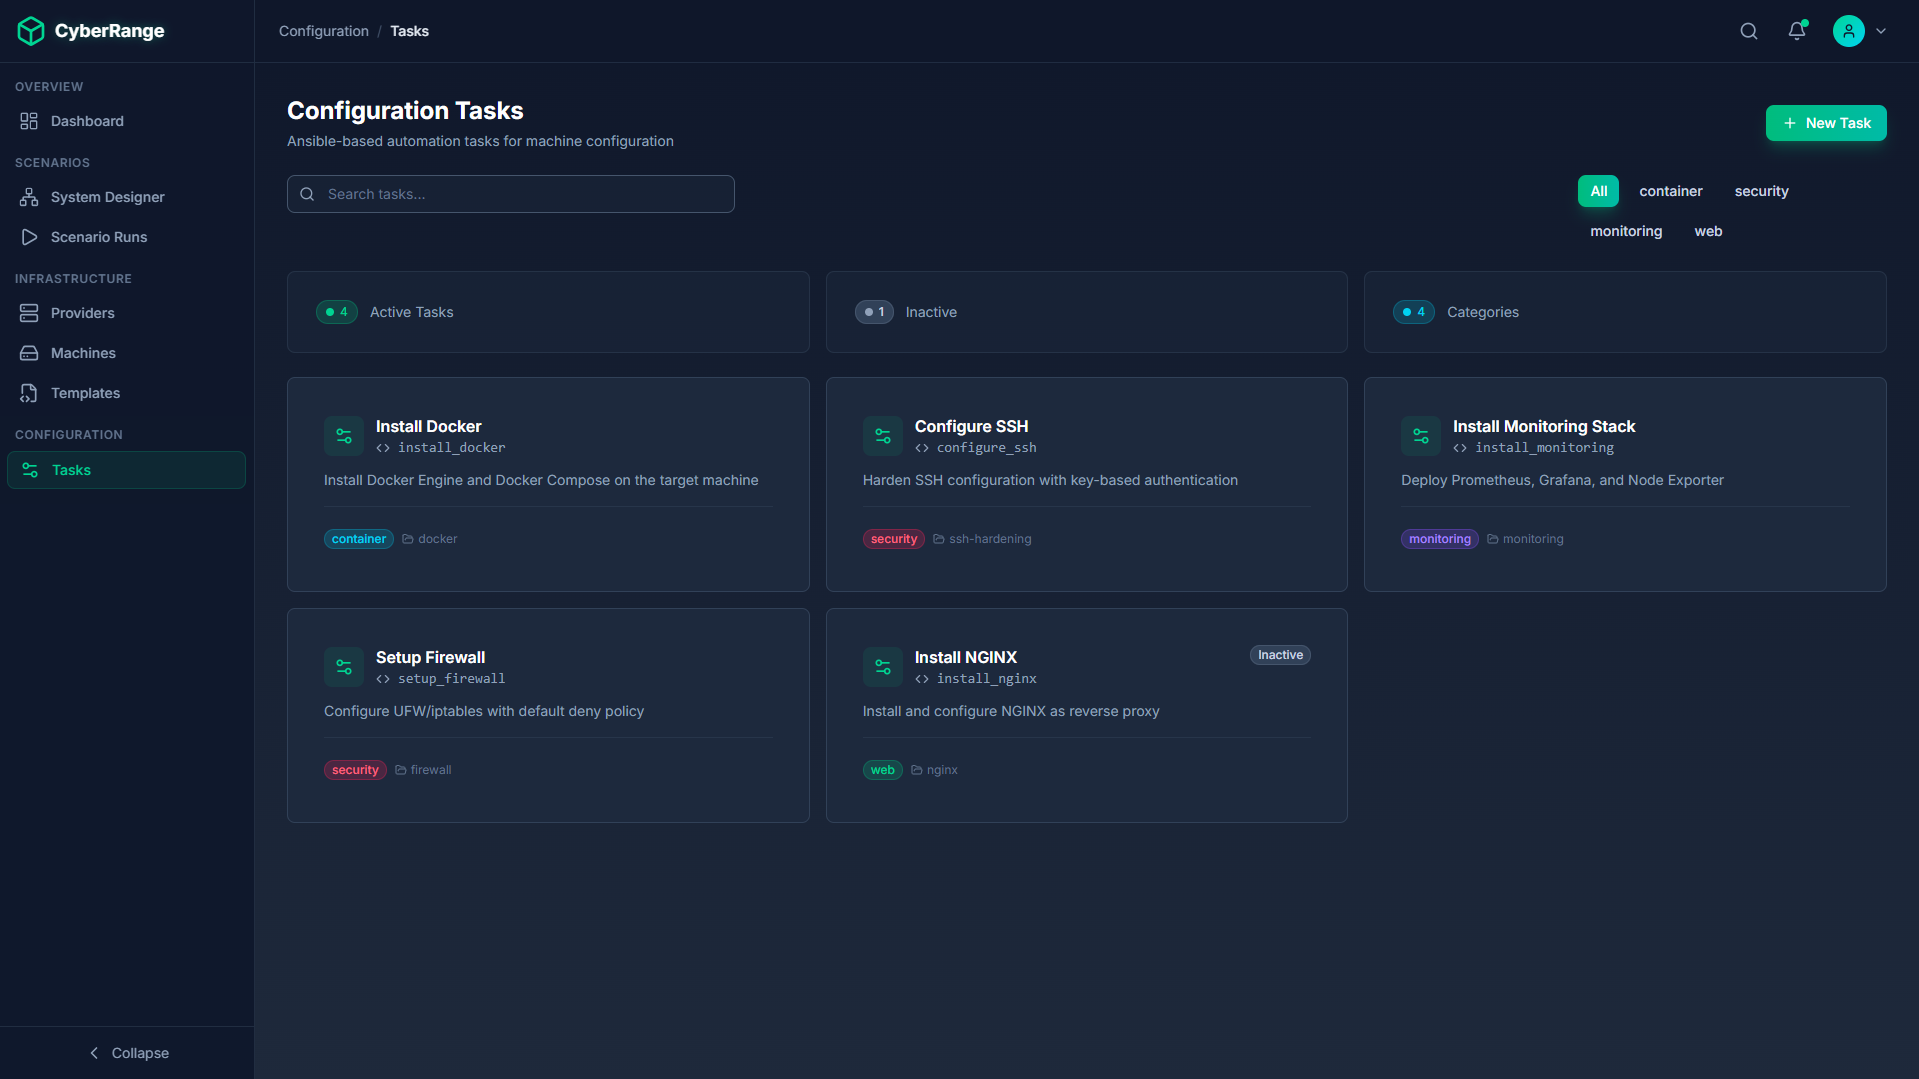
\includegraphics[width=0.95\textwidth]{images/wweb/tasks.png}
    \caption{Configuration task management.}
    \label{fig:phase5-task-management}
\end{figure}

\begin{figure}[H]
    \centering
    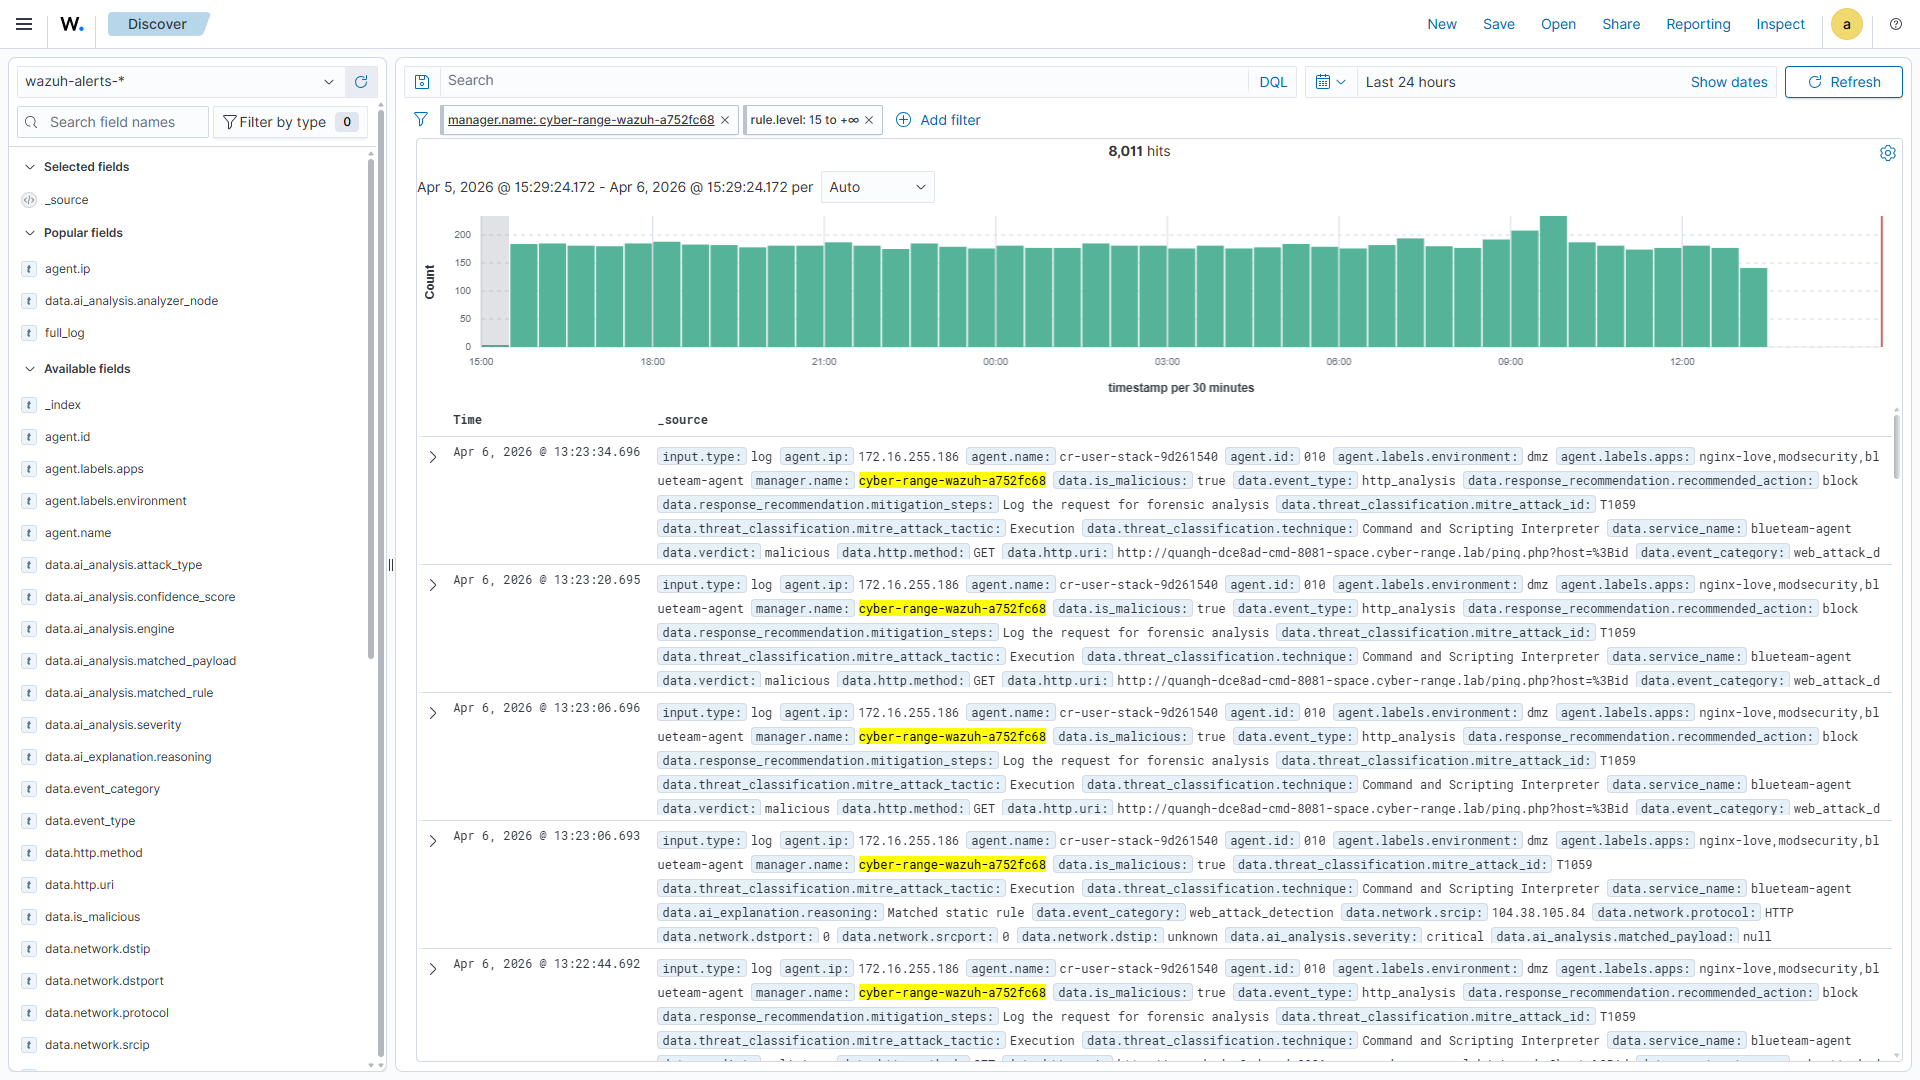
\includegraphics[width=0.95\textwidth]{images/wz.png}
    \caption{Wazuh log view.}
    \label{fig:wazuh-log-view-1}
\end{figure}

\begin{figure}[H]
    \centering
    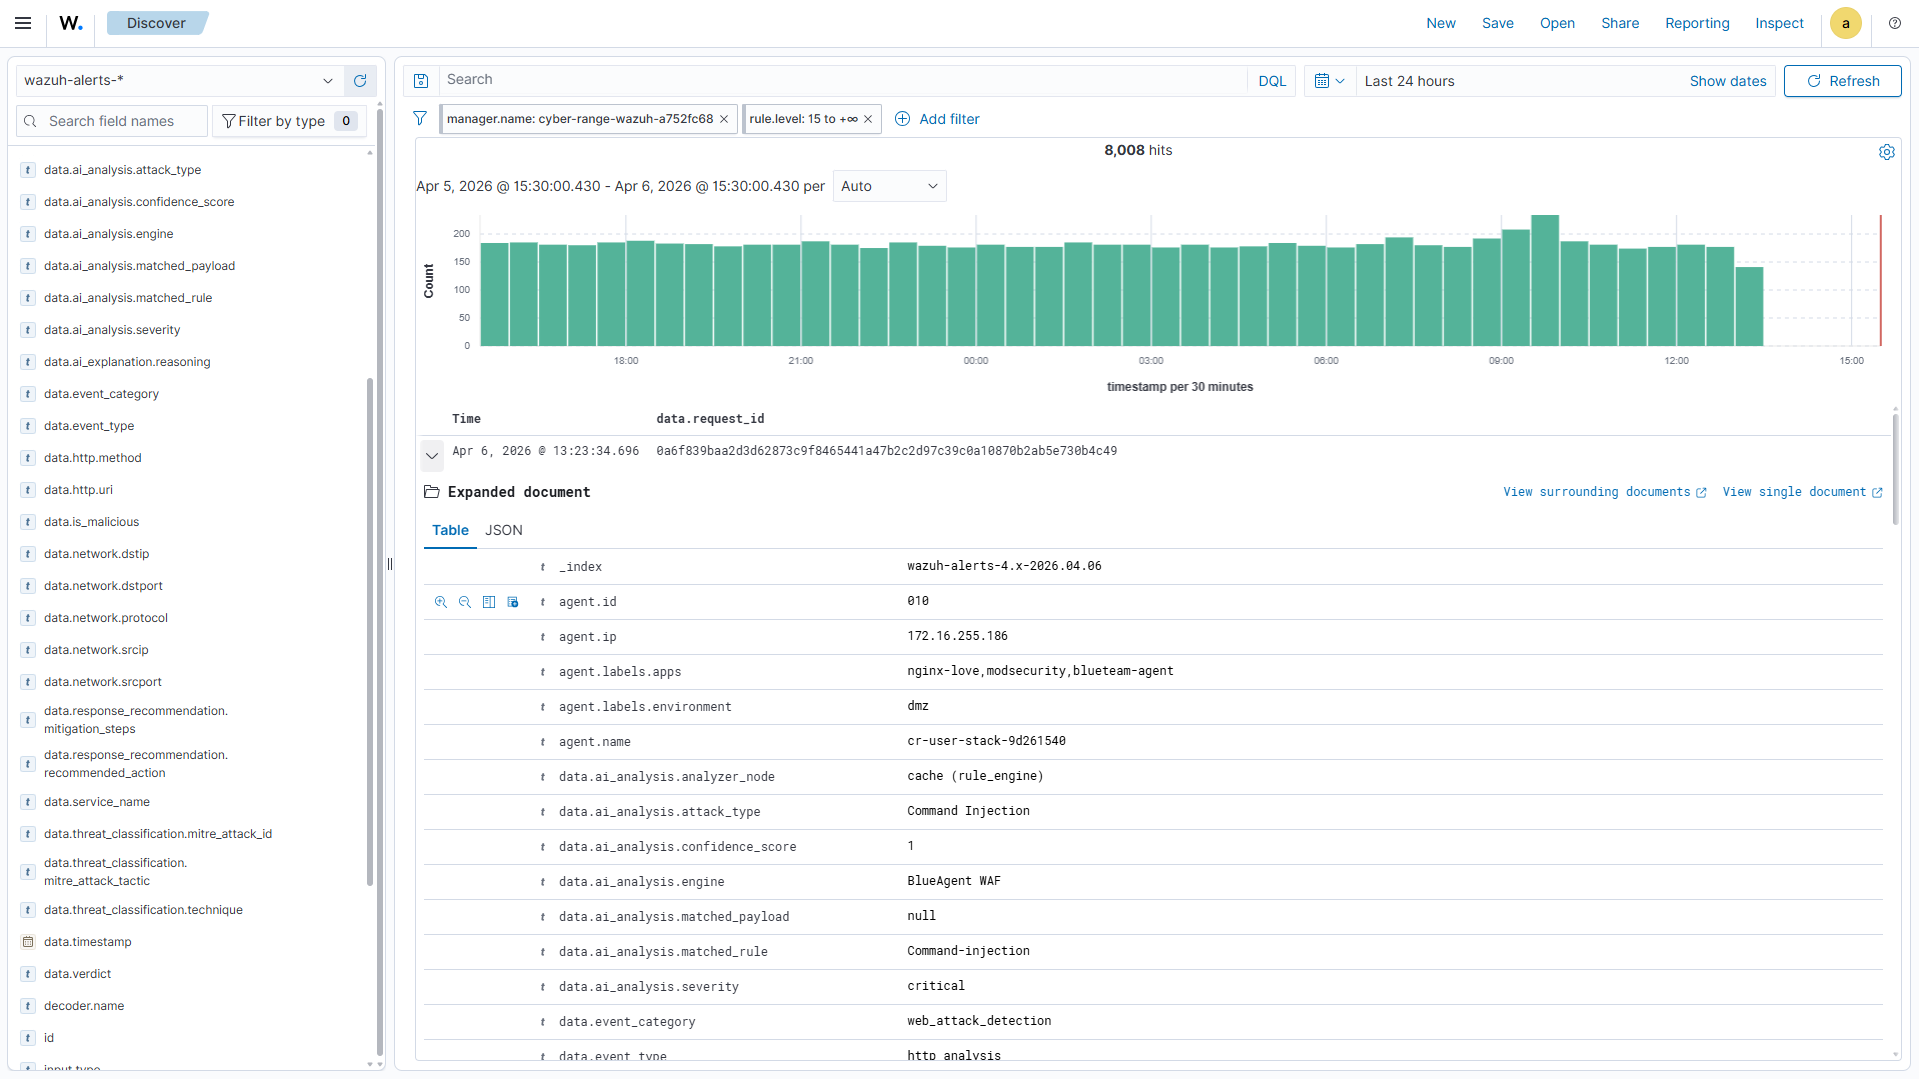
\includegraphics[width=0.95\textwidth]{images/wz1.png}
    \caption{Wazuh event details.}
    \label{fig:wazuh-log-view-2}
\end{figure}

\subsection{Phase 6: Dashboard Interaction and Visualization}
The objective of this phase was to integrate all operational capabilities into a coherent dashboard experience. Core functions included navigation across provider, template, scenario, deployment, and monitoring modules; state-aware data presentation; and role-appropriate interaction flows.

Practical usability is determined here. Even when backend services are correct, adoption in academic training depends on whether users can execute workflows efficiently through the dashboard interface.

In the implemented system, the dashboard is consolidated into a central operational overview page. This view summarizes infrastructure readiness and recent operator activity so that users can quickly assess platform state before creating scenarios or launching deployments.

The implemented dashboard workflow provides the following operational support:

\begin{enumerate}
    \item Presenting high-level platform metrics, including infrastructure providers, provisioned machines, validated templates, and active users.
    \item Exposing quick-action entry points for frequent administrative tasks such as adding providers, provisioning machines, and importing templates.
    \item Displaying recent activity events so that operators can verify successful actions, identify failed builds, and correlate changes with ongoing infrastructure work.
    \item Reducing navigation overhead by placing overview status, action shortcuts, and operational signals in one page.
\end{enumerate}

\begin{figure}[H]
    \centering
    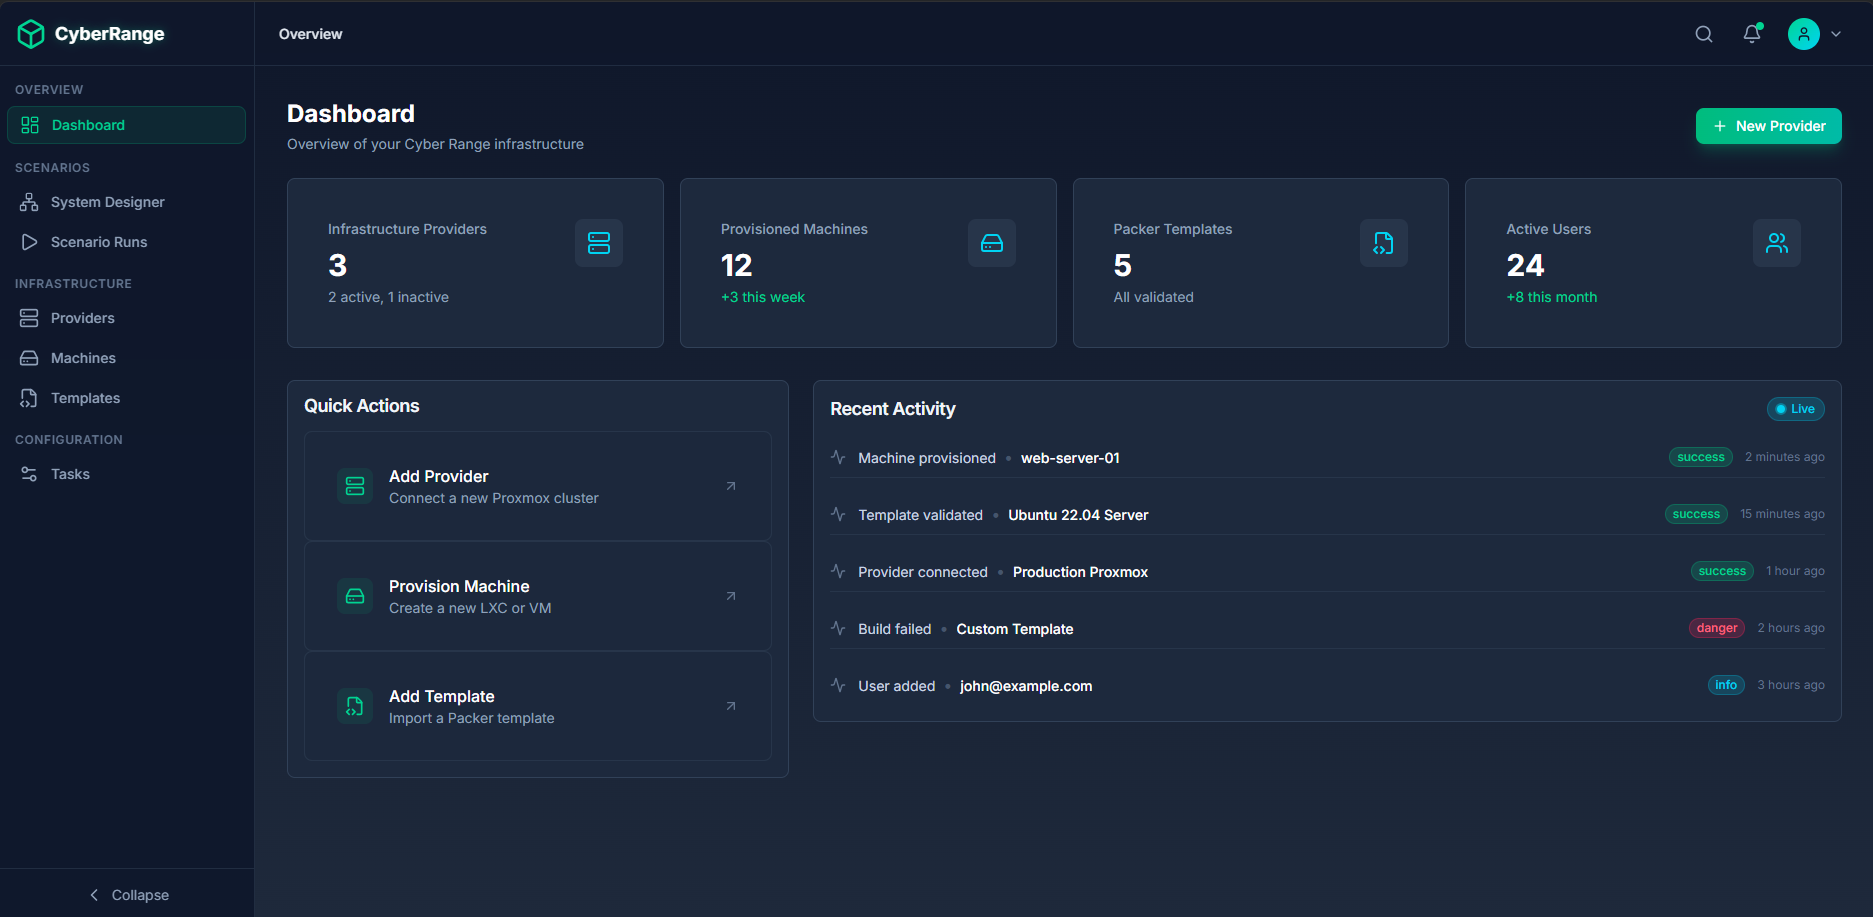
\includegraphics[width=0.95\textwidth]{images/dashboard/overview.png}
    \caption{Dashboard overview.}
    \label{fig:dashboard-overview-main}
\end{figure}

\subsection{Phase 7: AI-Assisted Analysis}
Where enabled, this phase introduced AI-assisted interpretation as an augmentation layer over system outputs. Core functions included contextual result summarization, explanatory assistance, request-level inspection, and support for training-oriented interpretation of operational or security-relevant events.

This phase plays a supporting rather than controlling role. The system remains governed by deterministic orchestration and monitored execution, while AI assistance improves interpretability and learning value. In the implemented project, the AI layer is exposed through a dedicated BlueAgent WAF console that supports request testing, alert review, and SOC-style copilot analysis in one workspace.

To improve factual grounding and reduce unsupported model responses, the project adopts a Retrieval-Augmented Generation (RAG) pattern inside the AI analysis pipeline. Rather than relying only on the internal knowledge of the language model, the system first retrieves relevant security context from a curated knowledge base and then injects that context into the final prompt. In this capstone, the retrieved context may include prior attack patterns, security explanations, rule descriptions, mitigation notes, and historical analyst guidance associated with web attacks such as SQL Injection, Cross-Site Scripting, and Path Traversal.

\subsubsection{RAG Overview}
In the context of this Cyber Range, RAG functions as an intermediate knowledge-enrichment layer between raw security events and final AI explanations. The objective is not only to classify a suspicious request, but also to provide a grounded explanation that is consistent with observed evidence and domain-specific references.

The adopted RAG architecture combines the following components:
\begin{itemize}
    \item \textbf{Input evidence:} raw HTTP requests, WAF alerts, selected SIEM fields, and request metadata collected from the training environment.
    \item \textbf{Embedding stage:} the incoming evidence and reference knowledge are transformed into vector representations using an embedding model.
    \item \textbf{Vector retrieval:} semantically similar knowledge chunks are retrieved from Qdrant based on the current request or alert.
    \item \textbf{Prompt augmentation:} the retrieved documents are merged with the observed request context and structured instructions.
    \item \textbf{Generation stage:} Gemini produces a final explanation, verdict, and mitigation-oriented interpretation using the grounded prompt.
    \item \textbf{Orchestration stage:} LangGraph coordinates retrieval, prompt assembly, fallback logic, and response formatting.
\end{itemize}

\begin{figure}[H]
    \centering
    
\includegraphics[width=0.9\textwidth]{images/RAG_pic.png}
    \caption{RAG-based analysis pipeline used in the AI-assisted security module.}
    \label{fig:rag-pipeline}
\end{figure}

\subsubsection{RAG Operational Flow}
The operational flow starts when a trainee or administrator submits a request to the BlueAgent WAF Console, or when the platform forwards a security-relevant event for interpretation. The backend first normalizes the request into a structured record that contains the request line, headers, payload fragments, WAF indicators, and scenario context. This normalization step is important because retrieval quality depends on consistent semantic representation of the evidence.

Next, the AI service generates an embedding for the normalized evidence and issues a similarity search against the vector database. Qdrant returns the most relevant knowledge chunks according to vector similarity. These chunks may describe known attack signatures, explain why a payload is suspicious, summarize WAF rule behavior, or provide mitigation advice that is useful for SOC-style training.

After retrieval, the orchestration layer filters irrelevant context, selects the top-ranked chunks, and combines them with the original request data. The final prompt therefore contains two complementary inputs: \textit{what happened in the current request} and \textit{what prior knowledge is most relevant to explain it}. Gemini then generates a grounded response that includes a verdict, confidence level, explanation, and investigation guidance. The generated output is finally returned to the dashboard for user review.

\clearpage
\subsubsection{Hybrid RAG-Based Payload Analysis Workflow}

Algorithm~\ref{alg:rag-analysis} presents the retrieval-augmented analysis workflow implemented in the system for HTTP payload inspection and security reasoning.

\begin{lstlisting}[caption={Hybrid RAG-based payload analysis workflow},label={alg:rag-analysis},basicstyle=\ttfamily\small,breaklines=true]
Input:
  raw_http_request R
  gatekeeper_model G
  vector_database V
  dense_embedding_model M
  sparse_retrieval_model B
  language_model L

Output:
  structured_security_analysis A

1. Parse R into structured HTTP components:
     method, URL, headers, and body
2. Extract user-controlled values from:
     URL path, query parameters, headers,
     cookies, form fields, and JSON body fields
3. Normalize extracted values into payload candidates P
4. Apply gatekeeper model G to identify suspicious payloads P_s
5. For each suspicious payload p in P_s:
     a. Encode p using dense embedding model M
     b. Construct a sparse BM25 query using model B
     c. Query vector database V using hybrid retrieval
        combining dense and sparse search
     d. Fuse retrieval results using reciprocal rank fusion (RRF)
6. Merge, deduplicate, and rank retrieved results
7. Select top-k payload intelligence snippets as context C
8. Construct augmented prompt P from:
     - suspicious payloads P_s
     - retrieved context C
     - analysis instructions
     - structured JSON output schema
9. Invoke language model L with prompt P
10. Generate verdict, attack classification, confidence,
      reasoning, and mitigation guidance
11. Return structured analysis A to the dashboard
\end{lstlisting}

From an implementation perspective, this workflow integrates hybrid retrieval over a Qdrant-based payload intelligence collection before invoking the language model. The retrieval stage combines dense semantic embeddings and sparse BM25 matching, followed by reciprocal rank fusion to improve relevance.

The retrieved context consists of known malicious payload patterns and labeled attack examples, which grounds the language model's reasoning in concrete evidence. This design reduces hallucination risk and improves both analytical accuracy and pedagogical value, making the system suitable for CyberRange training scenarios where explainability and contextual understanding are critical.

It should be noted that the vector database is constructed in an offline indexing phase, where payload intelligence data is normalized, embedded, and stored for efficient hybrid retrieval during inference.

To activate AI features, administrators configure Gemini integration from \texttt{Configuration $\rightarrow$ System Settings}. This workflow allows users to securely register API keys and manage global integration parameters used by AI-enabled agents.

\begin{enumerate}
    \item Open \texttt{System Settings} and select \texttt{New Setting}.
    \item Set \texttt{Category} to \texttt{ai} and define key name as \texttt{GEMINI\_API\_KEY}.
    \item Paste the Gemini API key in the \texttt{Value} field and provide a short description for maintenance.
    \item Enable \texttt{Active} to use this setting at runtime.
    \item Enable \texttt{Secret Value} so the key is stored encrypted in the database.
    \item Save the setting and verify it appears in the AI settings list.
\end{enumerate}

Once configured, the AI analysis console supports the following workflow:

\begin{enumerate}
    \item Select a quick test preset such as SQL Injection, Cross-Site Scripting, Path Traversal, or benign traffic.
    \item Submit a raw HTTP request to the analysis workspace for inspection.
    \item Allow the AI engine to return verdict, confidence, and explanation payloads for training interpretation.
    \item Use the same interface as a SOC copilot surface for guided investigation of request behavior and WAF outcomes.
\end{enumerate}

\begin{figure}[H]
    \centering
    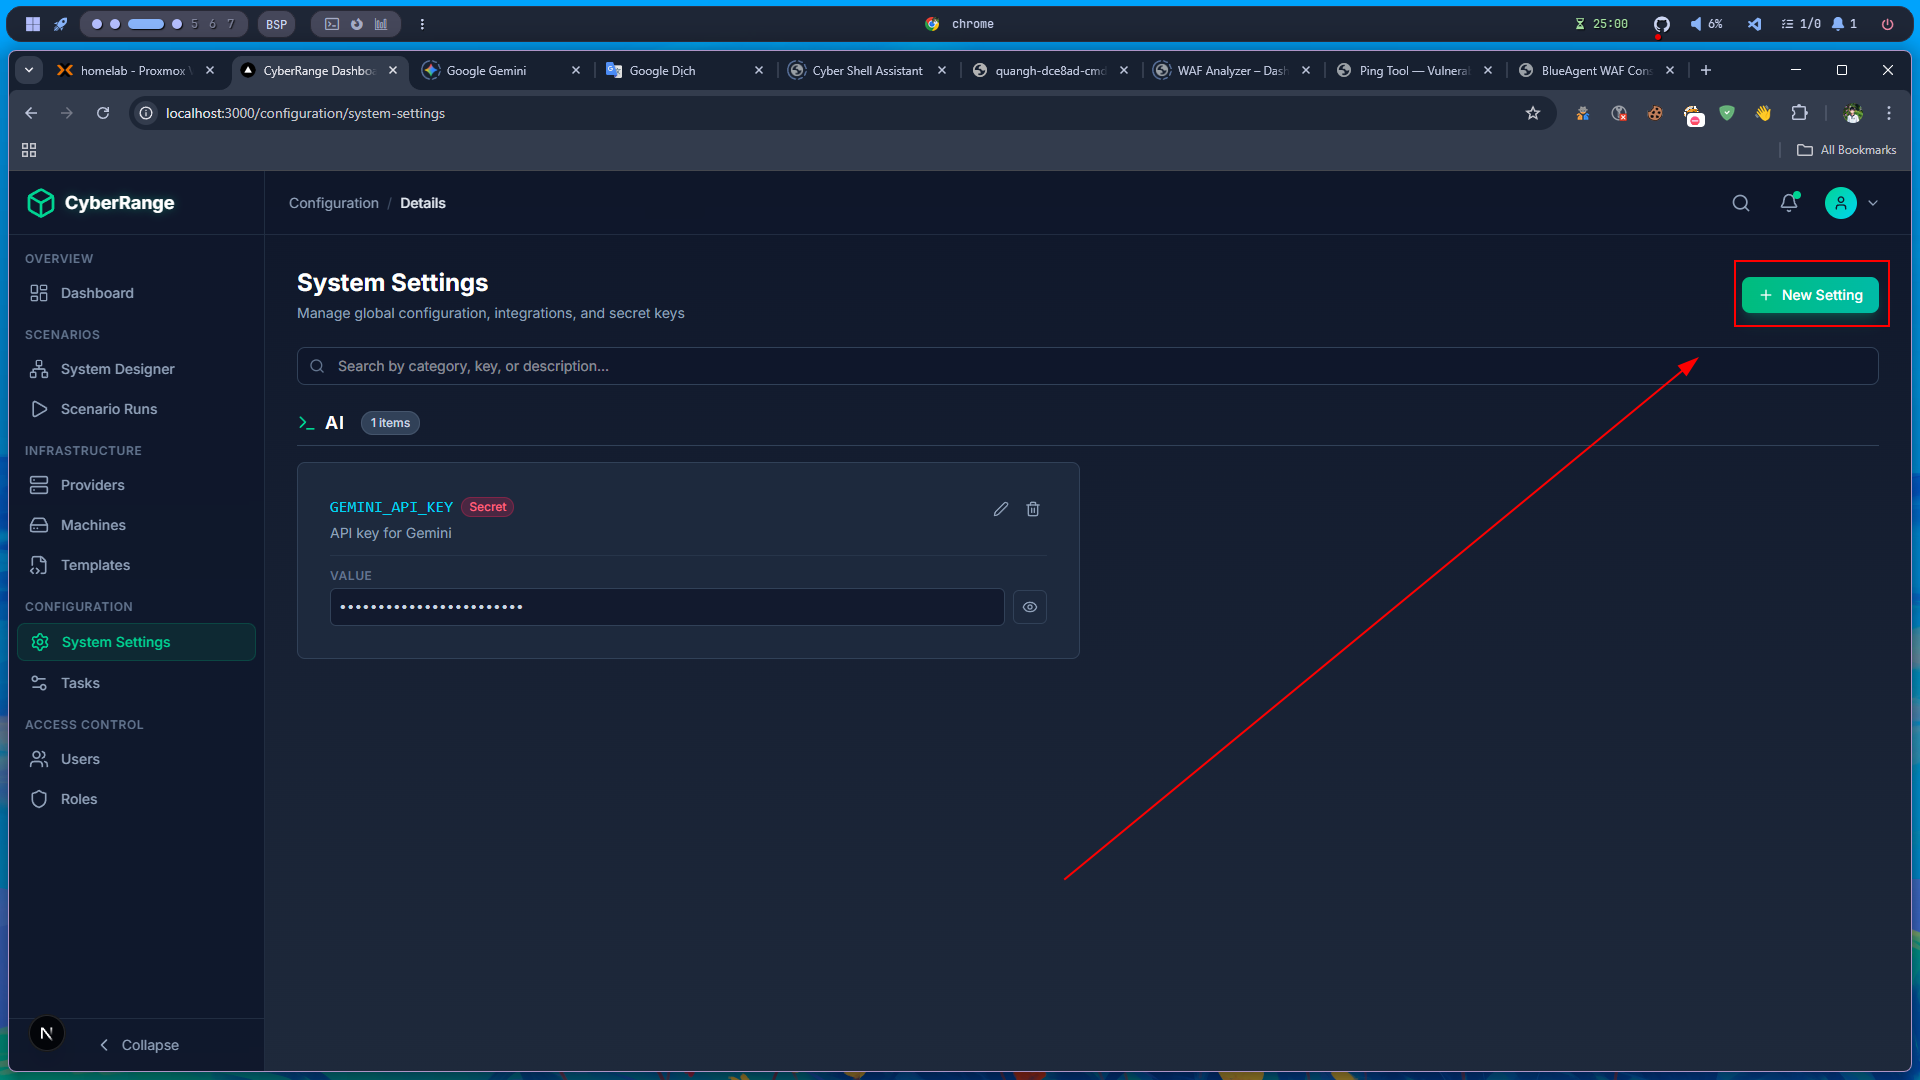
\includegraphics[width=0.95\textwidth]{images/settings/1.png}
    \caption{System settings view.}
    \label{fig:settings-gemini-list}
\end{figure}

\begin{figure}[H]
    \centering
    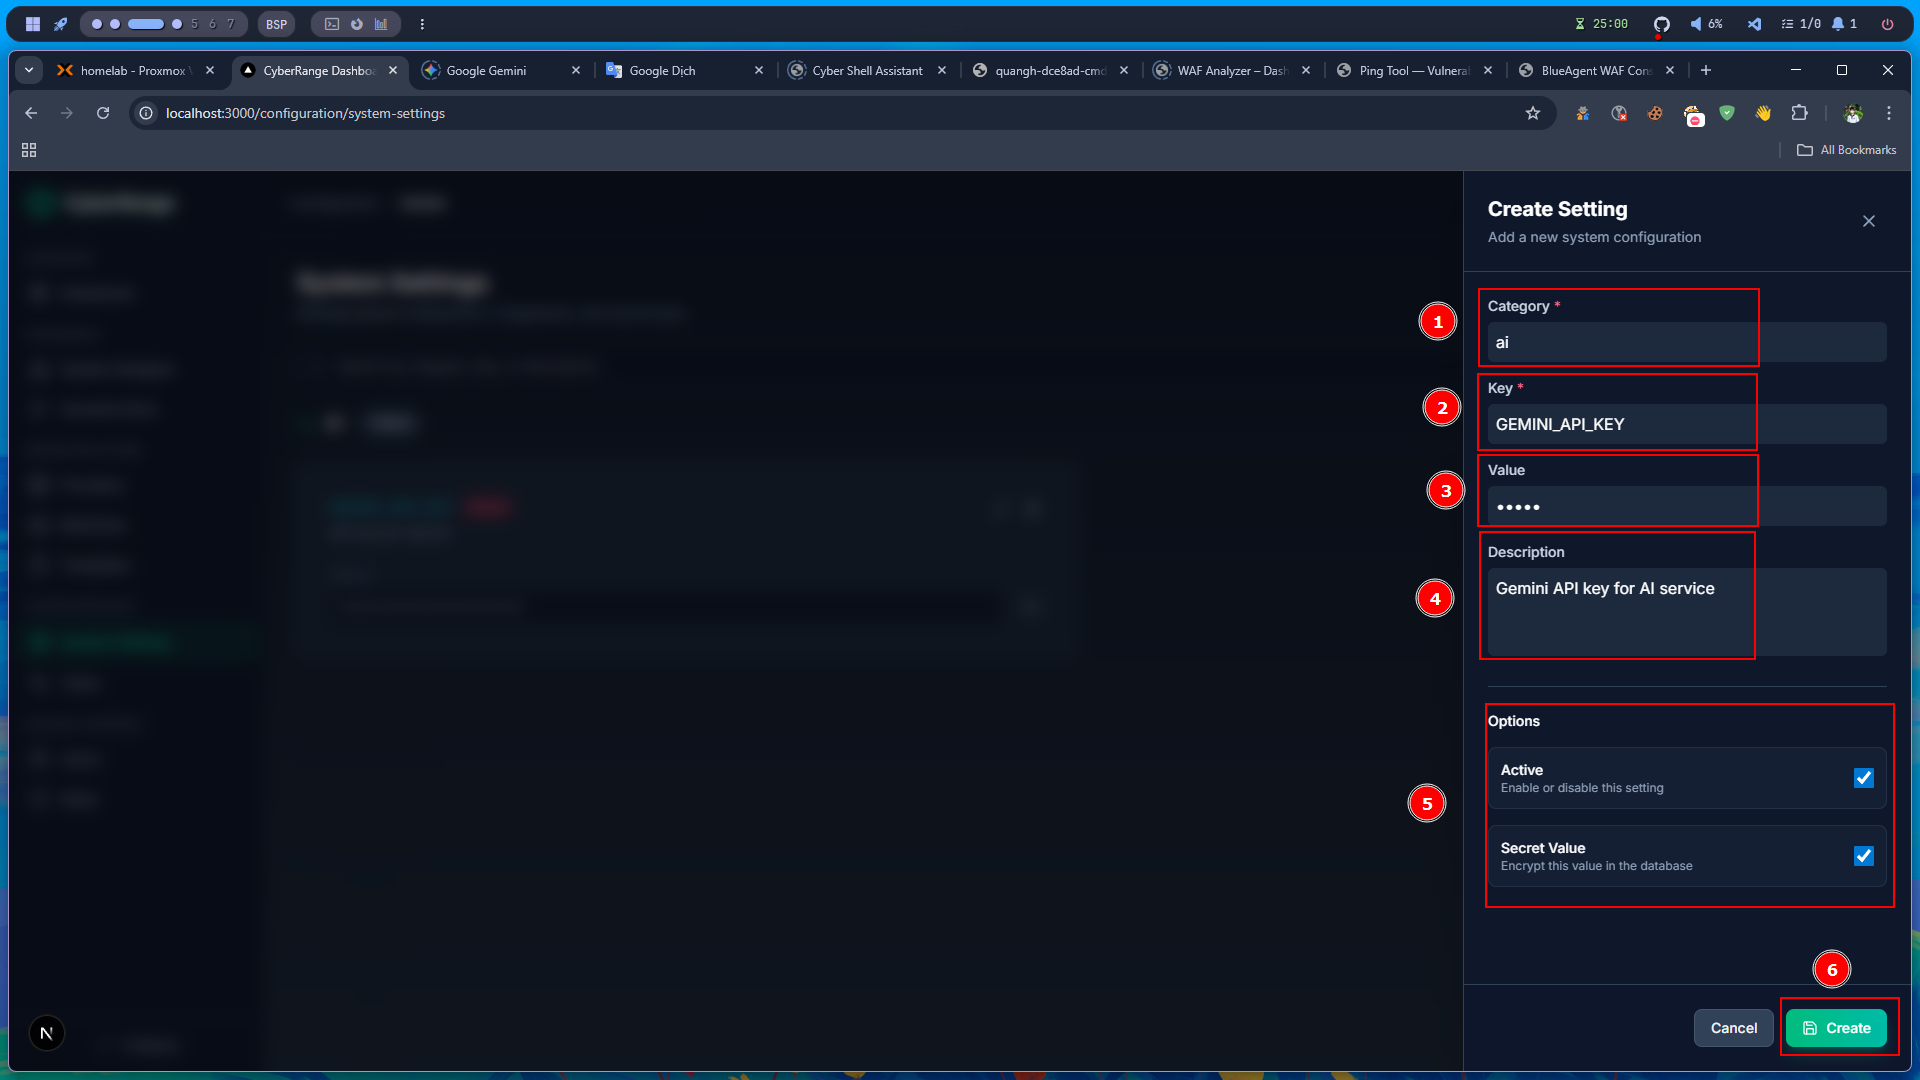
\includegraphics[width=0.95\textwidth]{images/settings/2.png}
    \caption{Gemini key setup form.}
    \label{fig:settings-gemini-create}
\end{figure}

\begin{figure}[H]
    \centering
    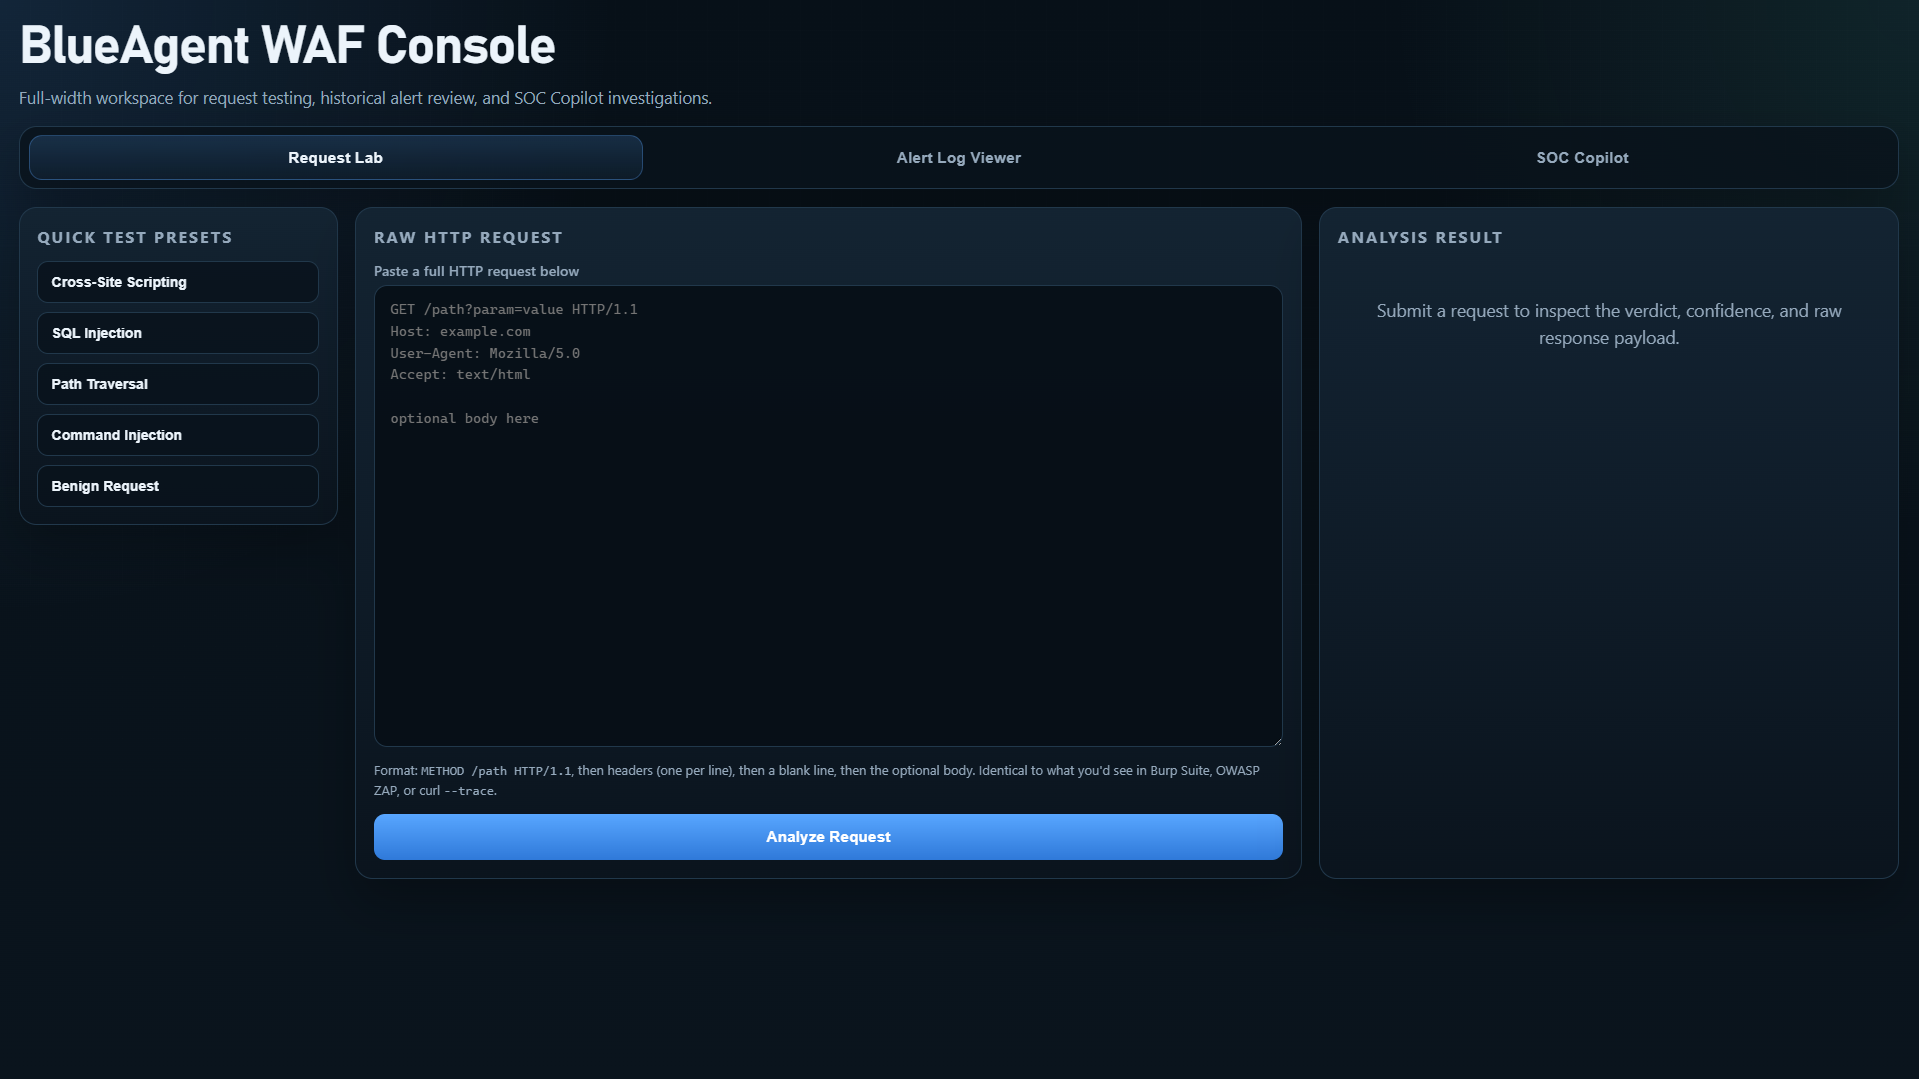
\includegraphics[width=0.95\textwidth]{images/wweb/AI analysis.png}
    \caption{BlueAgent WAF Console.}
    \label{fig:phase7-ai-console}
\end{figure}

\section{Implementation Timeline and Milestones}
\subsection{Milestone Definition}
Milestones were defined as integration-complete capabilities rather than isolated coding events. A milestone was considered achieved only when a feature could be executed from dashboard action to backend processing and observable result. This criterion ensured that progress reflected operational readiness, not only code availability.

Representative milestone groups included provider readiness, template/resource readiness, scenario lifecycle readiness, deployment orchestration readiness, monitoring readiness, and integrated dashboard readiness.

\subsection{Planned Timeline}
The timeline followed dependency order: provider setup preceded template preparation; templates preceded scenario definition; scenario definition preceded deployment validation; deployment validation preceded monitoring refinement and dashboard consolidation. AI-assisted analysis was positioned after baseline orchestration stability to ensure that interpretive features were added on top of a reliable execution core.

This sequence reduced rework, improved validation efficiency, and allowed each phase to inherit stable outputs from the previous phase.

\section{Resource and Responsibility Mapping}
\subsection{Team Responsibilities During Implementation}
Implementation responsibilities were assigned by functional domain to preserve accountability across system layers. Infrastructure-oriented responsibilities covered provider connectivity and deployment prerequisites. Application-oriented responsibilities covered scenario orchestration, task processing, and API behavior. Interface-oriented responsibilities covered dashboard workflow integrity and operational visibility. Validation-oriented responsibilities covered integration checks, defect tracking, and documentation quality.

This responsibility mapping enabled parallel work while maintaining clear ownership over cross-layer integration points.

\subsection{Infrastructure and Tooling Resources}
The implementation required resources for control services, data persistence, asynchronous task execution, and dashboard delivery. Tooling resources included provider integration utilities, template/resource management components, scenario lifecycle handlers, and monitoring/logging utilities for runtime observability.

From an academic deployment perspective, resource planning emphasized repeatability, controllability, and maintainable execution rather than maximal scale.

\section{Quality Assurance During Implementation}
\subsection{Coding and Integration Standards}
Quality control emphasized modular service boundaries, consistent API contracts, explicit error signaling, and deterministic state transitions for scenario lifecycle operations. Configuration handling and sensitive integration parameters were managed through controlled backend paths to reduce operational risk.

Integration standards required each module to expose observable outputs that could be validated through dashboard views and task logs.

\subsection{Verification and Validation Checkpoints}
Verification checkpoints were applied at the end of each phase to confirm that newly integrated capabilities remained compatible with existing workflows. Validation focused on end-to-end execution evidence: user action, backend processing, task-state progression, and observable result.

This checkpoint strategy reduced late-stage integration surprises and improved confidence in final demonstration readiness.

\section{Risks in Implementation Execution}
\subsection{Execution Risks}
Primary implementation risks included provider-connection instability, template inconsistency, scenario-definition mismatch, asynchronous job failure, incomplete observability in task logs, and user-flow ambiguity in dashboard navigation. Additional risk existed where AI-assisted outputs might be interpreted without sufficient contextual grounding.

\subsection{Mitigation Actions in Development}
Mitigation actions included staged integration, early validation of provider and template readiness, controlled scenario lifecycle testing, structured task/log monitoring, and retry-aware execution handling. Dashboard workflows were reviewed iteratively to reduce navigation ambiguity and improve operational clarity.

For AI-assisted functions, mitigation emphasized positioning AI outputs as advisory support, while retaining deterministic system control and traceable execution evidence.
